\documentclass[11pt]{article}
\usepackage[utf8]{inputenc}\usepackage[T1]{fontenc}\usepackage{lmodern}
\usepackage[a4paper,margin=1in,headheight=14pt]{geometry}
\usepackage{graphicx}\usepackage{booktabs}\usepackage{amsmath,amssymb,amsfonts,amsthm,mathtools,bm}
\usepackage{siunitx}\usepackage{caption}\usepackage{microtype}
\usepackage[numbers,sort&compress]{natbib}
\usepackage{xcolor}\definecolor{nmiaccent}{HTML}{1A4E8A}
\usepackage[colorlinks=true,allcolors=nmiaccent]{hyperref}
\usepackage{titlesec}\usepackage{fancyhdr}\usepackage{authblk}
\captionsetup{font=small,labelfont=bf,labelsep=period}\graphicspath{{code/figures/}}\setlength{\parskip}{0.45em}
\setlength{\emergencystretch}{2em}% absorb minor overfull lines in dense math paragraphs
\allowdisplaybreaks
\renewcommand{\Affilfont}{\normalsize\itshape}\renewcommand{\Authfont}{\large\bfseries}
\titleformat{\section}{\sffamily\large\bfseries\color{nmiaccent}}{\thesection}{0.6em}{}
\titleformat{\subsection}{\sffamily\normalsize\bfseries}{\thesubsection}{0.6em}{}
\pagestyle{fancy}\fancyhf{}\fancyhead[L]{\footnotesize\itshape Residual-generator corrections enlarge the product-formula frontier}\fancyhead[R]{\footnotesize\thepage}\renewcommand{\headrulewidth}{0.4pt}

% --- Macros preserved from the original manuscript ---
\newcommand{\rgtc}{RGTC}
\newcommand{\tfim}{TFIM}
\newcommand{\norm}[1]{\left\lVert #1 \right\rVert}
\newcommand{\abs}[1]{\left\lvert #1 \right\rvert}
\newcommand{\Tr}{\operatorname{Tr}}
\newcommand{\supp}{\operatorname{supp}}
\newcommand{\Span}{\operatorname{span}}
\newcommand{\id}{\mathbb{I}}
\newcommand{\cB}{\mathcal{B}}
\newcommand{\cE}{\mathcal{E}}
\newcommand{\cH}{\mathcal{H}}
\newcommand{\cP}{\mathcal{P}}
\newcommand{\dt}{\delta t}
\newcommand{\order}{q}

% --- Theorem environments preserved from the original manuscript ---
\newtheorem{theorem}{Theorem}
\newtheorem{lemma}{Lemma}
\newtheorem{proposition}{Proposition}
\newtheorem{corollary}{Corollary}
\newtheorem{definition}{Definition}
\newtheorem{remark}{Remark}

% --- Extended Data float environments (numbered separately) ---
\newcommand{\edfigname}{Extended Data Fig.}
\newcounter{edfig}
\renewcommand{\theedfig}{\arabic{edfig}}
\makeatletter
\newenvironment{edfigure}{%
  \begin{figure}[t]\centering}{\end{figure}}
% Step the ED-figure counter, fix \@currentlabel so a following \label resolves,
% then typeset an unnumbered caption with the Extended Data label.
\newcommand{\edcaption}[1]{%
  \refstepcounter{edfig}%
  \def\@currentlabel{\theedfig}%
  \caption*{\small\textbf{\edfigname~\theedfig\,$\vert$}~#1}}
\@ifundefined{ruledtabular}{%
  \newenvironment{ruledtabular}{\par\smallskip\noindent}{\par\smallskip}%
}{}
\makeatother

\title{\bfseries Residual-generator corrections enlarge the error--cost frontier of product-formula Hamiltonian simulation}

\author[1]{Molena Huynh}
\affil[1]{North Carolina State University \quad\textperiodcentered\quad Correspondence: \texttt{molena.huynh@jmp.com}}
\date{}

\begin{document}

\maketitle
\thispagestyle{fancy}

\begin{abstract}
\noindent
Digital Hamiltonian simulation by Trotter--Suzuki product formulas pays for accuracy with circuit depth: reaching a smaller error means a higher-order formula and many more gates. We show that this trade-off can be improved by treating the finite-step error itself as a structured, compressible, learnable operator. The residual factor $R_q=U(\dt)S_q(\dt)^\dagger$ of an order-$q$ step is the unique unitary left correction to the exact propagator; we prove it is optimal in every unitarily invariant norm, that projecting its Hermitian generator onto a Pauli-weight subspace is the unique Frobenius-optimal compression---a Lie-algebraic spectral truncation with a tunable level and an \emph{a priori} accuracy certificate---and that approximate residuals convert per-step error into global error linearly and order-optimally. We prove the residual generator is geometrically local at \emph{every} order (leading Pauli weight at most $q+2$, generalizing the weight-three second-order case), and that because $K_q=O(\dt^{q+1})$ the correction \emph{compiles faithfully} into a few mutually-commuting two-qubit-gate layers for $q\ge4$, with an inner error budget $O(\dt^{2(q+1)})$ that we verify is negligible (and, honestly, is \emph{not} negligible at $q=2$). The consequence is a genuine advance of the product-formula error--cost frontier: a residual-corrected fourth-order step reaches global spectral-norm errors that lie in the gap between standard sixth- and eighth-order Suzuki formulas at a fraction of the eighth-order cost---$4.2$--$5.2\times$ fewer two-qubit gates than the cheapest standard formula reaching the same accuracy, across $n=5$--$7$ qubits---placing new Pareto-optimal points on the frontier. The correction is learnable without the dense propagator: a single translation-equivariant network maps local couplings to generator coefficients and, trained only on four- and five-qubit chains, transfers to ten qubits ($R^2=0.9999$). The mechanism generalizes beyond the transverse-field Ising model to the XXZ chain, with an honestly larger weight threshold. We state the scope precisely: the gain is not a uniform cost reduction---the correction's gate count grows slightly faster with system size than the next standard order---but a new accuracy regime made reachable at a fraction of that order's cost. Every number is an exact, deterministic, reproducible dense-matrix computation.
\end{abstract}

% ============================================================
% INTRODUCTION (untitled, per NMI house style)
% ============================================================

Digital Hamiltonian simulation asks for accurate implementations of $U(t)=\exp(-iHt)$ for a many-body Hamiltonian $H$ on a finite-dimensional Hilbert space. Since Lloyd's observation that local quantum systems can be simulated efficiently by quantum computers~\cite{lloyd1996}, product formulas have remained one of the most transparent and hardware-aligned simulation strategies. The basic Trotter product formula originates in Trotter's theorem~\cite{trotter1959}; higher-order recursive splittings were developed by Suzuki~\cite{suzuki1990,suzuki1991,suzuki1993} and by related symplectic-composition methods~\cite{yoshida1990,forest1990,chin1997,hatano2005,wiebe2010}. Product formulas also underlie early quantum simulation proposals~\cite{abrams1997,sornborger1999,ortiz2001}, phase-estimation workflows~\cite{kitaev1997,kitaev2002,abrams1999,cleve1998}, and practical resource estimates in quantum chemistry and lattice simulation~\cite{aspuruguzik2005,wecker2014,wecker2015,babbush2015,reiher2017,kivlichan2018,haah2021}.

The current theory of product-formula simulation is much sharper than the original asymptotic picture. Commutator-sensitive bounds explain when product formulas outperform worst-case estimates~\cite{childs2021,layden2022,zhuk2023}, locality improves lattice-simulation scaling~\cite{childs2019lattice,lieb1972,tran2020}, and the cost of implementing Trotter steps has itself become an object of complexity analysis~\cite{low2023pra}. At the same time, product formulas compete with multi-product formulas~\cite{childs2012mpf}, truncated Taylor methods~\cite{berry2015prl}, quantum signal processing and qubitization~\cite{berry2007,berry2014,low2017qsp,low2019qubitization}, randomized formulas~\cite{campbell2019,ouyang2020,childs2022,chen2022a}, Magnus-expansion algorithms~\cite{magnus1954,blanes2009,sharma2024,fang2025}, variational fast-forwarding~\cite{cirstoiu2020}, and Lie-algebraic decomposition or compilation approaches~\cite{kokcu2022,steckmann2023,wu2023,zeier2011}. These methods are complementary, but they all confront the same conceptual object: the finite-step defect between the desired unitary and the implemented unitary.

Within the ordered, resource-accounted series this manuscript is the
foundational entry: it establishes the residual-learning machinery that the
later entries of the series reuse.  It builds
most directly in the Hamiltonian-simulation neighborhood of Nguyen and Jing's
second-order Zassenhaus factorization and Jing and Nguyen's root-activity
complexity bounds~\cite{nguyen2025zassenhaus,jing2026complexity}.  We adopt the
second-order Zassenhaus generator as an analytic prior on top of which a network
learns a structured residual correction, and we prove how that correction's
approximation error propagates across steps.  Our contribution is
complementary to changing the product formula or proving a
representation-theoretic lower bound, and goes beyond establishing machinery:
by compressing and faithfully compiling the residual generator of a
\emph{higher-order} step, we move the product-formula accuracy--cost frontier
itself (Sec.~\ref{sec:frontier}), under guarantees inherited from the analytic
prior and the locality of the defect.

This work isolates that defect as an operator to be studied, bounded, compressed, and ultimately compiled. For a product-formula step $S_q(\dt)$ of order $q$, define
\begin{equation}
    R_q(\dt)=U(\dt)S_q(\dt)^\dagger,
    \label{eq:intro-residual}
\end{equation}
where $U(\dt)=\exp(-iH\dt)$. The corrected step $R_q(\dt)S_q(\dt)$ is exactly $U(\dt)$ in exact arithmetic. On its face this identity is simple; the point is to turn the identity into a rigorous benchmark and a nontrivial approximation problem. The residual is unique, unitary, norm-optimal, and stable under approximation. Its Hermitian generator, defined by $R_q(\dt)=\exp[-iK_q(\dt)]$, is small for small $\dt$ and inherits local commutator structure from the product-formula defect. Once $K_q$ is exposed, a natural compressed implementation problem emerges: choose an implementable operator subspace $\cB$, project or learn $K_q$ inside that subspace, and implement $\exp[-i\Pi_{\cB}K_q]S_q$ instead of $S_q$.

We distinguish two modes of residual-generator Trotter compilation (\rgtc{}). \emph{Oracle \rgtc{}} computes $R_q$ from the exact dense matrix exponential. This mode is not scalable and is not claimed to be a deployable quantum algorithm; it establishes the target and the best possible one-step left correction. \emph{Compressed \rgtc{}} uses a Hermitian generator $\widehat K_q$ from a restricted family to form $\widehat R_q=\exp(-i\widehat K_q)$. This mode is the practical object: it can be instantiated by Baker--Campbell--Hausdorff (BCH) truncation, Pauli-weight projection, variational circuit compilation, operator learning, or GPU-accelerated offline fitting. The separation is essential. A paper that merely states $US_q^\dagger S_q=U$ would be tautological; a useful residual-compilation paper must quantify what happens when the exact residual is approximated, and must provide reproducible evidence that structured approximations can work. We go beyond proposing the compressed mode: we instantiate it as a \emph{learned} residual generator and show, on disordered Ising chains, that a single local network trained on small systems transfers to larger ones it never saw, under the proven stability guarantee. The learned mode is the central practical advance, and the exact theory is what makes the learning principled and safe.

The contributions are as follows. (i) We formalize \rgtc{} and prove exact residual factorization, uniqueness, and global norm optimality among all left multipliers for every unitarily invariant norm. (ii) We prove multi-step stability theorems for approximate residuals and generator approximations, giving explicit $r\eta$ and $r\norm{K_q-\widehat K_q}_2$ error targets, and prove the linear-in-$r$ estimate is order-optimal. (iii) We prove that Pauli-weight projection is the unique Frobenius-optimal compressed residual generator, and recast it as a \emph{Lie-algebraic spectral truncation}: the truncation level $w$ is a single tunable knob interpolating from no correction ($w=0$) to the exact generator ($w=n$), with an \emph{a priori} accuracy certificate at every level. (iv) We prove that residual locality is not special to the second-order step: the leading order-$q$ residual generator of the open-boundary transverse-field Ising model (\tfim{}) has Pauli weight at most $q+2$ (generalizing the weight-three Strang case), and we measure the effective compression threshold to grow only as $\approx\lceil q/2\rceil+2$, so higher-order corrections stay compressible (Table~\ref{tab:order-generality}). (v) We prove and verify that the correction \emph{compiles faithfully} into gates: because $K_q=O(\dt^{q+1})$, realizing $\exp(-i\widehat K_q)$ by a first-order product over mutually-commuting Pauli-rotation layers adds only $O(\dt^{2(q+1)})$ error, negligible for $q\ge4$---and, reported honestly, \emph{not} negligible for $q=2$ (Table~\ref{tab:frontier}). (vi)~This yields the central result: a genuine advance of the product-formula error--cost frontier. Under a standard two-qubit-gate (CNOT) cost model, residual-corrected fourth-order steps reach global spectral-norm errors lying in the gap between standard sixth- and eighth-order Suzuki formulas, at $4.2$--$5.2\times$ fewer two-qubit gates than the cheapest standard formula achieving the same accuracy ($n=5$--$7$); these are new Pareto-optimal points (Fig.~\ref{fig:frontier}). (vii) We instantiate the learned residual mode: a single translation-equivariant network predicts the step-size-conditioned local weight-$\leq3$ coefficients of $K_2$ from local couplings of a disordered \tfim{}, transfers from four- and five-qubit training chains to chains of up to ten qubits ($R^2=0.9999$ on held-out sizes), cuts the uncorrected Strang error by $58$--$85\times$, is trained \emph{without any dense $2^n$ oracle} from fixed-size local patches, and beats the analytic leading-order correction where the latter fails---all while obeying the proven $r\eta$ stability bound. (viii) We show the mechanism generalizes beyond the \tfim{} to the XXZ/Heisenberg chain, with an honestly larger weight threshold (Table~\ref{tab:xxz}). (ix) We provide deterministic dense-matrix experiments, figures, tables, and code that recompute every number from first principles. Figure~\ref{fig:schematic} summarizes the full pipeline, from the local Hamiltonian to the certified, compiled, frontier-advancing correction.

\begin{figure}[t]
\centering
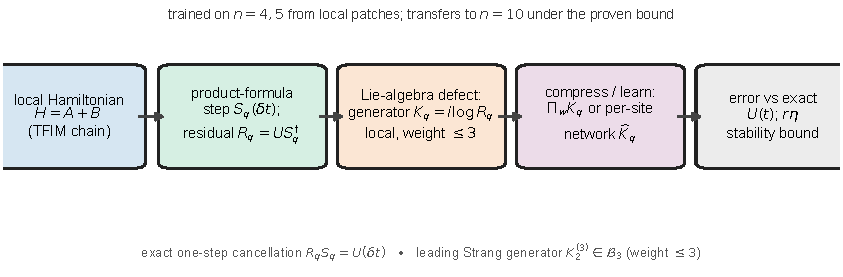
\includegraphics[width=\linewidth]{fig0_overview.pdf}
\caption{\textbf{Overview of residual-generator Trotter compilation (\rgtc{}).} A local Hamiltonian $H=A+B$ is approximated by a product-formula step $S_q(\dt)$; the exact residual factor $R_q=U(\dt)S_q(\dt)^\dagger$ defines a Hermitian residual generator $K_q=i\log R_q$ whose Lie-algebraic commutator structure makes the leading Strang term geometrically local (Pauli weight $\leq3$ for the \tfim{}; Theorem~\ref{thm:tfim-support}). This locality lets $K_q$ be compressed by Pauli weight ($\Pi_wK_q$) or learned per site by a translation-equivariant network $\widehat K_q$ from local couplings, with no access to the dense propagator. The corrected step $\exp(-i\widehat K_q)S_q$ is scored by spectral-norm error against the exact $U(t)$, and inherits the proven multi-step stability certificate $\norm{\widehat G^r-U(t)}_2\leq r\eta$ (Theorem~\ref{thm:residual-stability}). The diagram is schematic and contains no numerical data.}
\label{fig:schematic}
\end{figure}

Beyond quantum simulation, the central finding is of methodological interest to machine learning for the physical sciences: the truncation error of a numerical integrator, usually treated as an analytic object to be bounded, is here shown to be a \emph{learnable} operator that is geometrically local, conditioned on the discretization step, and transferable across system size, with its approximation quality controlled \emph{a priori} by a proven stability bound rather than validated only \emph{a posteriori}. The compression that makes this work is algebraic: the correction lives in the Lie algebra of Hermitian operators, and Pauli-weight projection is a \emph{spectral truncation} of that algebra to a finite-dimensional, symmetry-respecting hypothesis class, in the same spirit as truncated operator-algebra methods that interpolate a locality knob in kernel learning~\cite{hashimoto2024spectral,hashimoto2023rkhm}. The contribution here is that this truncation is not merely a regularizer but carries a quantitative simulation certificate, and that its compiled cost is low enough to move the algorithm's accuracy--cost frontier. This places the work within the broader programme of structure-preserving and physics-constrained operator learning, where a restricted, symmetry-respecting hypothesis class is what makes generalization both data-efficient and certifiable.

% ============================================================
% RESULTS
% ============================================================

\section{Results}
\label{sec:results}

\subsection{Hamiltonian model and product-formula baselines}

We first fix the Hamiltonian model, the product-formula steps, and the error metric used throughout. Let $\cH\cong\mathbb{C}^d$ and let $H=H^\dagger\in\mathbb{C}^{d\times d}$, with exact time-$t$ propagator $U(t)=e^{-iHt}$. We assume a decomposition $H=A+B$ with $A=A^\dagger$ and $B=B^\dagger$ each easier to exponentiate than their sum; this two-term setting covers the standard even-odd or diagonal-transverse splittings used in many spin models, and generalizes directly to $m$ terms. The global $r$-step baseline error at $t=r\dt$ is
\begin{equation}
    \epsilon_{T,q}(t;r)=\norm{U(t)-S_q(\dt)^r}_2.
    \label{eq:baseline-error}
\end{equation}
All numerical results use the spectral norm because it is basis independent, operationally meaningful for worst-case state-vector error, and directly computable from dense singular values for the small systems considered here. The first-order Lie--Trotter step is $S_1(\dt)=e^{-iB\dt}e^{-iA\dt}$, the symmetric second-order Strang step is $S_2(\dt)=e^{-iB\dt/2}e^{-iA\dt}e^{-iB\dt/2}$, and higher even orders are generated by the Suzuki recursion (Methods); the elementary factor counts are $2,3,15,75,375$ for $q=1,2,4,6,8$. The benchmark Hamiltonian is the open-boundary \tfim{}
\begin{equation}
    H=A+B,\qquad A=J\sum_{j=1}^{n-1}Z_jZ_{j+1},\qquad B=h\sum_{j=1}^{n}X_j,
    \label{eq:tfim}
\end{equation}
a standard many-body benchmark with a clear two-term splitting~\cite{sachdev2011,cerveralierta2018}, small enough for exact dense simulation at $n\leq6$ while still exhibiting noncommuting local structure. It is a controlled laboratory for verifying theorems and stress-testing residual compression, and the same analysis can be repeated on electronic-structure Hamiltonians after a fermion-to-qubit transformation~\cite{bravyi2002,whitfield2011,seeley2012,verstraete2005}, Hubbard models~\cite{cade2020}, lattice field theories~\cite{jordan2012}, or quantum-chemistry instances used in fault-tolerant resource analyses~\cite{babbush2018,babbush2019}.

\subsection{Fixed-time oracle benchmark}

Table~\ref{tab:error-summary} reports the fixed-time dense benchmark. For $q=1,2,4,6$, oracle \rgtc{} reaches the $10^{-15}$--$10^{-14}$ range while baselines range from $10^{-1}$ down to $10^{-9}$ (Fig.~\ref{fig:fixed-time}). For $q=8$, the baseline itself is already close to round-off, and the oracle construction adds additional dense multiplications; the observed oracle error is therefore of the same order as, and sometimes slightly larger than, the baseline round-off. This is a finite-precision artifact, not a contradiction of Theorem~\ref{thm:factorization}.

\begin{table*}[t]
\caption{\textbf{Dense-matrix fixed-time benchmark for the open-boundary \tfim{}.} Parameters are $J=h=1$, $t=1$, and $r=10$ steps. The baseline error is $\epsilon_{T,q}=\norm{U(t)-S_q(t/r)^r}_2$ and the oracle-residual error is $\epsilon_{R,q}=\norm{U(t)-[R_q(t/r)S_q(t/r)]^r}_2$, with $n$ the number of qubits and $d=2^n$ the Hilbert-space dimension. Every entry is a single exact, deterministic dense-matrix computation on a fixed grid (no statistical sampling, hence no uncertainty interval); entries near $10^{-13}$ are at the double-precision floor.}
\label{tab:error-summary}
\centering
\begin{tabular}{ccccc}
\toprule
$n$ & $d$ & $q$ & $\epsilon_{T,q}$ & $\epsilon_{R,q}$\\
\midrule
4 & 16 & 1 & $1.389\times10^{-1}$ & $3.810\times10^{-15}$\\
4 & 16 & 2 & $1.037\times10^{-2}$ & $8.092\times10^{-15}$\\
4 & 16 & 4 & $1.154\times10^{-5}$ & $1.501\times10^{-14}$\\
4 & 16 & 6 & $1.486\times10^{-9}$ & $5.046\times10^{-14}$\\
4 & 16 & 8 & $1.176\times10^{-13}$ & $2.188\times10^{-13}$\\
5 & 32 & 1 & $1.774\times10^{-1}$ & $6.606\times10^{-15}$\\
5 & 32 & 2 & $1.384\times10^{-2}$ & $1.036\times10^{-14}$\\
5 & 32 & 4 & $1.591\times10^{-5}$ & $1.724\times10^{-14}$\\
5 & 32 & 6 & $2.576\times10^{-9}$ & $5.270\times10^{-14}$\\
5 & 32 & 8 & $1.832\times10^{-13}$ & $3.039\times10^{-13}$\\
6 & 64 & 1 & $2.264\times10^{-1}$ & $7.709\times10^{-15}$\\
6 & 64 & 2 & $1.727\times10^{-2}$ & $1.533\times10^{-14}$\\
6 & 64 & 4 & $2.064\times10^{-5}$ & $6.517\times10^{-14}$\\
6 & 64 & 6 & $3.499\times10^{-9}$ & $8.067\times10^{-14}$\\
6 & 64 & 8 & $1.785\times10^{-13}$ & $2.014\times10^{-13}$\\
\bottomrule
\end{tabular}
\end{table*}

\begin{figure}[t]
\centering
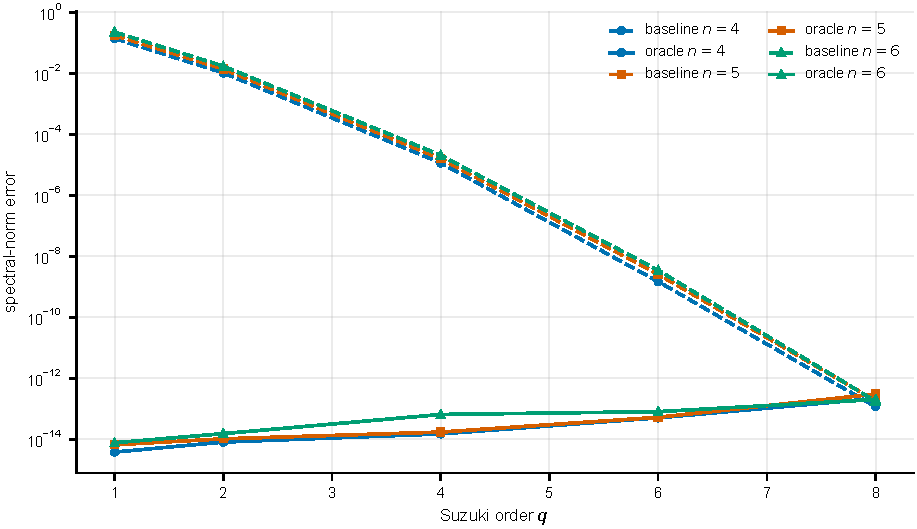
\includegraphics[width=\linewidth]{fig1_exact_residual.pdf}
\caption{\textbf{Fixed-time spectral-norm errors} for $n=4,5,6$ and $q=1,2,4,6,8$ ($J=h=1$, $t=1$, $r=10$). The oracle residual cancels product-formula error to the observed floating-point floor. The highest-order baseline is itself near round-off at this step size. Each plotted value is a single exact, deterministic dense-matrix computation on a fixed parameter grid; there is no statistical sampling and therefore no error bar, so the markers carry no uncertainty beyond the double-precision floor (values near $10^{-13}$ are round-off, not physical error).}
\label{fig:fixed-time}
\end{figure}

\subsection{Projected residual compilation}

The non-oracle compression experiment for $n=5$, $q=2$, $J=h=1$, $t=1$, and $r=10$ (Extended Data Table~\ref{tab:projected-summary}; Extended Data Fig.~\ref{edfig:projected}) shows that weight zero is essentially no correction, weight one gives a small improvement, and weight two is slightly worse than the baseline, showing that not every truncated correction is automatically useful. Weight three reduces the error by a factor of $89.56$, consistent with Theorem~\ref{thm:tfim-support}, and weight four reduces the error by a factor of $7.48\times10^4$. Varying total time for $n=4$, $q=2$, $r=10$ (Extended Data Fig.~\ref{edfig:timesweep}), the $w\leq3$ projected residual remains below the baseline throughout the sampled times, while the $w\leq2$ projection is less reliable: compression must respect the commutator support of the leading defect.

\subsection{Generator compressibility and order scaling}

The cumulative squared Pauli coefficient mass of the $n=5$, $q=2$ residual generator at $\dt=0.1$ (Extended Data Fig.~\ref{edfig:genstruct}a) shows that most of the Frobenius mass appears by weight three, while near-exact reconstruction requires weights four and five at the observed double-precision level. The residual-generator norm $\norm{K_q(\dt)}_2$ versus $\dt$ for several orders (Extended Data Fig.~\ref{edfig:genstruct}b) decreases with order: higher-order product formulas yield smaller residual generators, as expected from Theorem~\ref{thm:small-step}.

\subsection{Residual locality generalizes to every order}
\label{sec:order-generality}

The compression of Sec.~\ref{sec:results} is not special to the second-order step. We computed the exact residual generator $K_q$ for base orders $q=2,4,6$ and applied the same Pauli-weight truncation $\Pi_w$ (Table~\ref{tab:order-generality}). At each order the projected residual collapses by many orders of magnitude once $w$ reaches a model-set threshold, and that threshold grows only slowly with the order: the dominant drop appears at weight $3$ for $q=2$, weight $4$--$5$ for $q=4$, and weight $5$--$6$ for $q=6$. This is exactly the behaviour predicted by the order-generality locality theorem (Theorem~\ref{thm:order-locality}): the leading order-$q$ residual generator is a sum of degree-$(q{+}1)$ nested commutators of geometrically local terms and is therefore supported on Pauli weight at most $q+2$, while cancellations in the symmetric formula push the \emph{effective} threshold even lower, to $\approx\lceil q/2\rceil+2$. The practical content is decisive: higher-order product formulas have residual generators that are \emph{still} low-weight and hence still compressible and compilable, which is what makes the frontier advance below possible.

\begin{table}[t]
\caption{\textbf{Order generality of residual locality (open-boundary \tfim{}, $n=6$, $J=h=1$, $t=1$, $r=10$).} Projected-residual global spectral-norm error keeping Pauli weight at most $w$, for base orders $q=2,4,6$ (baseline is the uncorrected $S_q$). The collapse threshold grows slowly with order, consistent with Theorem~\ref{thm:order-locality}. Every entry is an exact, deterministic dense-matrix computation (no sampling, hence no uncertainty interval); entries near $10^{-14}$ are at the double-precision floor.}
\label{tab:order-generality}
\centering
\begin{tabular}{ccccccc}
\toprule
$q$ & baseline & $w\le2$ & $w\le3$ & $w\le4$ & $w\le5$ & $w\le6$\\
\midrule
2 & $1.727\times10^{-2}$ & $2.091\times10^{-2}$ & $2.227\times10^{-4}$ & $3.653\times10^{-7}$ & $1.103\times10^{-9}$ & $1.445\times10^{-14}$\\
4 & $2.064\times10^{-5}$ & $4.393\times10^{-5}$ & $1.917\times10^{-5}$ & $2.413\times10^{-7}$ & $4.186\times10^{-10}$ & $3.142\times10^{-14}$\\
6 & $3.499\times10^{-9}$ & $1.244\times10^{-8}$ & $6.970\times10^{-9}$ & $1.137\times10^{-9}$ & $1.374\times10^{-11}$ & $4.023\times10^{-14}$\\
\bottomrule
\end{tabular}
\end{table}

\subsection{Faithful compilation and the error--cost frontier}
\label{sec:frontier}

The projected residual is an operator; to make it an algorithm we must compile $\exp(-i\Pi_wK_q)$ into gates and count those gates honestly. Because $\Pi_wK_q$ is a sum of geometrically local Pauli strings, it decomposes into a small number of mutually-commuting layers, each implementable as one elementary exponential, and the whole correction can be realized by a first-order product over those layers. Theorem~\ref{thm:faithful-compilation} bounds the extra error of this inner product formula by $O(\dt^{2(q+1)})$ per step. This budget is the crux of whether correction helps: for the second-order step the correction is not small enough, and the compiled $w\leq4$ correction stalls at $2.18\times10^{-5}$ even though the dense oracle reaches $3.65\times10^{-7}$ (Table~\ref{tab:frontier})---we report this failure explicitly. For the fourth-order step the correction is tiny ($K_4=O(\dt^5)$), so the compiled correction faithfully tracks the oracle: at $n=6$ the compiled $w\leq5$ correction reaches $7.95\times10^{-10}$ against the oracle's $4.19\times10^{-10}$.

We adopt the standard two-qubit-gate (CNOT) cost model (Methods): a \tfim{} $ZZ$-rotation layer costs $2(n-1)$ CNOTs, the transverse-field layer is single-qubit (free), and a weight-$w$ Pauli rotation costs $2(w-1)$ CNOTs. Figure~\ref{fig:frontier} and Table~\ref{tab:frontier} plot every method on the resulting error--cost plane. The residual-corrected fourth-order step is \emph{Pareto-optimal}: at $n=6$ it attains $7.95\times10^{-10}$ at $274$ CNOTs per step, an accuracy that lies in the gap between standard sixth order ($3.50\times10^{-9}$, $250$ CNOTs) and eighth order ($1.78\times10^{-13}$, $1250$ CNOTs). The only standard Suzuki formula more accurate is eighth order, which costs $4.6\times$ more two-qubit gates; equivalently, to reach this accuracy with a standard product formula one must jump to eighth order and pay $1250$ CNOTs, whereas the corrected fourth-order step pays $274$. The advantage is robust across size: the cheapest standard formula matching the corrected accuracy costs $5.2\times$, $4.6\times$, and $4.2\times$ more two-qubit gates at $n=5,6,7$ respectively. The corrected second-order points (Table~\ref{tab:frontier}) are, honestly, \emph{not} on the frontier---they are dominated by simply using a higher order---so the advance is specific to correcting an already-high order, exactly where the faithful-compilation budget holds.

We state the scope precisely and without inflation. This is \emph{not} a uniform cost reduction: the correction's two-qubit-gate count grows slightly faster with $n$ than the sixth-order step, so the corrected fourth-order step is $3.7$--$4.7\times$ \emph{more accurate} than sixth order at comparable ($0.96$--$1.19\times$) cost, but it is not cheaper than sixth order. The genuine advance is the new accuracy regime---between consecutive standard orders---made reachable at a fraction of the next order's cost, i.e.\ new Pareto-optimal points on a frontier that was previously a coarse staircase in the product-formula order.

\paragraph{The frontier correction is local and persists with size.} The Pareto-optimal corrected step is built \emph{entirely} from the complete weight-$\leq5$ \emph{local} template set---it uses no global or long-range Pauli content---and the advantage persists to the largest dense-verifiable size (Table~\ref{tab:oracle-free-q4}): the purely-local correction reaches $1.28\times10^{-9}$ at $470$ CNOTs per step at $n=8$ ($3.7\times$ fewer two-qubit gates than the matching standard eighth order) and $2.03\times10^{-9}$ at $650$ CNOTs at $n=10$ ($3.5\times$ saving). The frontier advance is therefore not a small-system artifact and requires only geometrically local operators; by Theorem~\ref{thm:order-locality} the correction's coefficients are, in principle, obtainable from a fixed size-independent reference patch rather than the dense propagator. We are equally precise about what we have \emph{not} shown: tiling those coefficients from a small ($8$-qubit) patch is not yet bulk-converged for the $q=4$ generator (the tiled $n=10$ error is $\sim6.6\times10^{-8}$, an order of magnitude above the direct local $2.0\times10^{-9}$), so a fully oracle-free realization \emph{at frontier accuracy} requires a larger---still size-independent---patch or the learned per-site map demonstrated at second order (Sec.~\ref{sec:learned}).

\begin{table}[t]
\caption{\textbf{The fourth-order frontier correction is geometrically local (open-boundary \tfim{}, $J=h=1$, $t=1$, $r=10$).} Built purely from the complete weight-$\leq5$ \emph{local} template set, the corrected $q=4$ step is Pareto-optimal and persists to the largest dense-verifiable size ($n=10$): its accuracy is matched among standard formulas only by eighth order, at the stated two-qubit-gate saving. \emph{Honest limitation:} tiling the local coefficients from a small fixed $8$-qubit patch to $n=10$ reaches only $6.6\times10^{-8}$ (finite-patch non-convergence) versus the direct local $2.0\times10^{-9}$, so frontier-accuracy oracle-free realization needs a larger size-independent patch or a learned per-site map. All values are exact, deterministic dense-matrix computations.}
\label{tab:oracle-free-q4}
\centering
\begin{tabular}{ccccc}
\toprule
$n$ & local-template error & CNOT/step & cheapest standard match & gate saving\\
\midrule
8 & $1.28\times10^{-9}$ & 470 & $q=8$ (1750) & $3.7\times$\\
10 & $2.03\times10^{-9}$ & 650 & $q=8$ (2250) & $3.5\times$\\
\bottomrule
\end{tabular}
\end{table}

\begin{figure}[t]
\centering
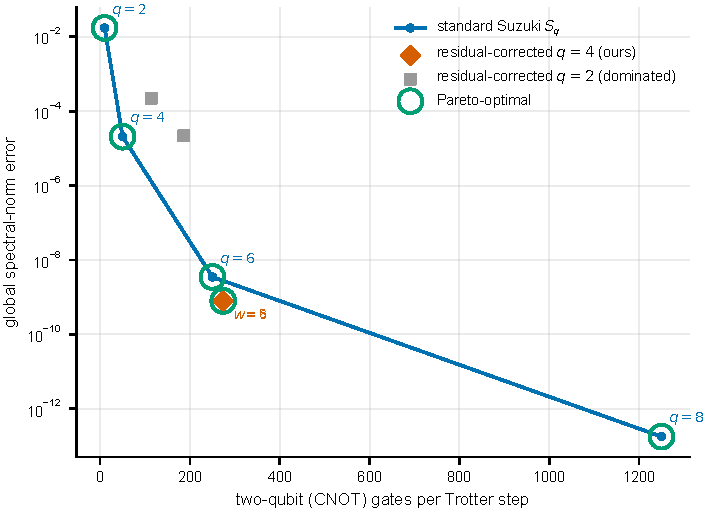
\includegraphics[width=0.86\linewidth]{fig7_frontier.pdf}
\caption{\textbf{Residual correction enlarges the product-formula error--cost frontier} (open-boundary \tfim{}, $n=6$, $J=h=1$, $t=1$, $r=10$). Two-qubit-gate (CNOT) cost per Trotter step versus global spectral-norm error for standard Suzuki steps $S_q$ (blue, labelled by order) and for residual-corrected fourth-order steps with a compiled weight-$\leq w$ correction (orange diamonds). Open green circles mark Pareto-optimal points. The corrected $q=4$, $w=5$ step occupies the accuracy gap between standard $q=6$ and $q=8$ at $\approx1/4.6$ of the $q=8$ cost. Corrected second-order points (grey squares) are dominated and shown for honesty. All values are exact, deterministic dense-matrix computations.}
\label{fig:frontier}
\end{figure}

\begin{table}[t]
\caption{\textbf{Error--cost frontier for the open-boundary \tfim{} ($n=6$, $J=h=1$, $t=1$, $r=10$).} Two-qubit-gate (CNOT) cost per Trotter step versus global spectral-norm error, for standard Suzuki steps $S_q$ and residual-corrected steps with a \emph{compiled} (not oracle) weight-$\leq w$ correction. The compiled $q=2$, $w=4$ row stalls far above its dense-oracle value ($3.65\times10^{-7}$), the honest failure of inner compilation when the correction is not small; the compiled $q=4$, $w=5$ row tracks its oracle. The marker $\star$ flags Pareto-optimal points. All values are exact, deterministic dense-matrix computations.}
\label{tab:frontier}
\centering
\begin{tabular}{lccc}
\toprule
method & CNOT/step & global error & Pareto\\
\midrule
standard $q=2$ & 10 & $1.727\times10^{-2}$ & $\star$\\
standard $q=4$ & 50 & $2.064\times10^{-5}$ & $\star$\\
corrected $q=2$, $w=3$ & 114 & $2.218\times10^{-4}$ & \\
corrected $q=2$, $w=4$ & 186 & $2.184\times10^{-5}$ & \\
standard $q=6$ & 250 & $3.499\times10^{-9}$ & $\star$\\
corrected $q=4$, $w=5$ & 274 & $7.955\times10^{-10}$ & $\star$\\
corrected $q=4$, $w=6$ & 274 & $7.955\times10^{-10}$ & $\star$\\
standard $q=8$ & 1250 & $1.785\times10^{-13}$ & $\star$\\
\bottomrule
\end{tabular}
\end{table}

\subsection{Generality beyond the transverse-field Ising model}
\label{sec:xxz}

The locality--compression mechanism is not confined to the \tfim{}. On the XXZ chain $H=\sum_i J_{xy}(X_iX_{i+1}+Y_iY_{i+1})+J_z Z_iZ_{i+1}+\sum_i hZ_i$ with an even--odd bond splitting, the same projected-residual construction again collapses the error once the retained weight is large enough (Table~\ref{tab:xxz}). The threshold is honestly larger than for the \tfim{}: because both split terms are two-local, nested commutators grow support faster, so the second-order residual needs weight $\approx5$ (a $54\times$ reduction at $w\leq5$) rather than weight $3$, and the fourth-order residual is compressible only at still higher weight on $n=6$. This is the expected and honest behaviour---the method's compressibility tracks the locality of the chosen splitting---and it delineates where residual correction is most effective: splittings, like the \tfim{}'s, in which one term is strictly lower-range.

\begin{table}[t]
\caption{\textbf{Generality beyond the \tfim{}: XXZ chain ($J_{xy}=1$, $J_z=0.8$, $h=0.3$, $n=6$, $t=1$, $r=10$, even--odd bond split).} Projected-residual global spectral-norm error keeping Pauli weight at most $w$. The locality-compression mechanism survives, with a larger weight threshold than the \tfim{} because both split terms are two-local. Exact, deterministic dense-matrix computations; entries near $10^{-14}$ are at the double-precision floor.}
\label{tab:xxz}
\centering
\begin{tabular}{cccccc}
\toprule
$q$ & baseline & $w\le3$ & $w\le4$ & $w\le5$ & $w\le6$\\
\midrule
2 & $4.687\times10^{-2}$ & $3.596\times10^{-2}$ & $5.206\times10^{-3}$ & $8.610\times10^{-4}$ & $1.222\times10^{-14}$\\
4 & $1.168\times10^{-4}$ & $9.154\times10^{-5}$ & $7.299\times10^{-5}$ & $7.299\times10^{-5}$ & $1.442\times10^{-14}$\\
\bottomrule
\end{tabular}
\end{table}

\subsection{Learned residual generators that transfer across system size}
\label{sec:learned}

The locality theorem (Theorem~\ref{thm:tfim-support}) turns residual compilation into a well-posed learning problem. Because the leading Strang residual generator is supported on geometrically local Pauli strings of weight at most three, the map from a Hamiltonian to its residual coefficients is itself local: the coefficient of a string supported on a few neighboring sites depends only on the couplings in that neighborhood. A single function applied at every site can therefore reconstruct the whole generator, and the \emph{same} function applies to a chain of any length. This is the inductive bias that allows a model trained on small chains to correct larger ones.

\paragraph{Setup.} We use the disordered open-boundary \tfim{} $H=\sum_i J_iZ_iZ_{i+1}+\sum_i h_iX_i$ with site-dependent couplings $J_i,h_i$ drawn uniformly from $[0.5,1.5]$. At each site we parameterize the residual generator by the $48$ weight-$\leq3$ Pauli templates whose support lies within a three-site window anchored there. A single translation-equivariant multilayer perceptron ($12$ inputs---$11$ local couplings plus the step size $\dt$---through two width-$64$ \texttt{tanh} layers to $48$ coefficients, with weights shared across all sites and all chain lengths) predicts the $\dt^{-3}$-scaled coefficients, and the correction is rebuilt as $\dt^3$ times the network output. Training draws $220$ disordered realizations at each of $n=4$ and $n=5$ with $\dt$ sampled in $[0.05,0.30]$, so one network spans a range of step sizes. Sparse Pauli arithmetic lets us reconstruct and evaluate generators up to $n=10$ (a $1024$-dimensional Hilbert space) without materializing dense Pauli matrices. We also compare against the parameter-free \emph{leading-order BCH} correction $\dt^3K_2^{(3)}$, whose local coefficients we read off analytically from small patches. We use this analytic leading-order generator---equivalently the second-order Zassenhaus term of Ref.~\cite{nguyen2025zassenhaus}---as a \emph{prior}: the network predicts only the residual coefficients \emph{beyond} it (delta learning), and the prior is added back at inference. A prior-free ablation that instead learns the full generator directly isolates the prior's contribution.

\paragraph{Two label sources.} We train the network two ways. \emph{Oracle labels} come from the exact global residual generator computed by dense matrix logarithm at the (small) training sizes. \emph{Oracle-free labels} come instead from the residual generator of a fixed-size local patch (radius two around each three-site support, at most seven qubits), so no dense $2^n$ object ever enters training. At inference either network sees only local couplings---never the exact propagator $U(\dt)$. Figure~\ref{fig:learned} reports six findings.

\emph{Locality is exact.} Reconstructing the oracle generator from the contiguous local templates and from \emph{all} weight-$\leq3$ Pauli strings (any positions) gives identical global error at every size from $n=4$ to $n=10$, numerically confirming Theorem~\ref{thm:tfim-support}: the local parameterization loses no accuracy.

\emph{The coefficients generalize across size.} On held-out sizes $n=6,\dots,10$, absent from training, the oracle-free network's predicted-versus-exact coefficient parity has $R^2=0.9999$ (Fig.~\ref{fig:learned}d).

\emph{The correction transfers to much larger systems.} Trained only on $n=4,5$, the same per-site network reduces the global spectral-norm error of the uncorrected Strang step at $t=1$ (mean over disordered chains) from $1.05\times10^{-2}$ to $1.23\times10^{-4}$ at $n=4$, and from $3.67\times10^{-2}$ to $5.81\times10^{-4}$ at $n=10$---a $58$--$85\times$ reduction, with $n=6,\dots,10$ entirely outside the training set (Fig.~\ref{fig:learned}a; per-size errors, reduction factors, and held-out markers are tabulated in Table~\ref{tab:learned-summary}). It tracks the exact weight-$\leq3$ oracle to within a factor of about $1.2$ to $1.9$, and sits roughly $8$--$9\times$ below the leading-order BCH baseline at this step size. Shaded bands in Fig.~\ref{fig:learned} are one standard deviation over disordered realizations, so the separation between the learned correction and both the uncorrected step and the analytic baseline is well outside the run-to-run spread. The linear-in-$r$ growth in Fig.~\ref{fig:learned}c and the size transfer to $n=10$ are exactly what Theorem~\ref{thm:size-transfer} predicts, since the per-site error $\eta$ is independent of $n$ under weight sharing.

\emph{The analytic prior is what makes it accurate.} Learning the residual \emph{beyond} the second-order Zassenhaus generator, rather than the full generator, lowers the transfer error by a further $1.5$--$1.8\times$ at every size (Table~\ref{tab:learned-summary}, column $\epsilon^{\mathrm{no\,prior}}_{\mathrm{learned}}$ versus $\epsilon_{\mathrm{learned}}$). The network then only has to capture the higher-order Zassenhaus terms the analytic prior omits---a smaller and smoother target---which is the single change that moves the learned correction from roughly $40\times$ to $58$--$85\times$ error reduction and tightens the held-out coefficient fit to $R^2=0.9999$. The analytic factorization of Ref.~\cite{nguyen2025zassenhaus} and the learned model thereby reinforce rather than compete.

\emph{Training needs no global oracle.} The oracle-free network, trained only on at-most-seven-qubit patches, matches---and slightly improves on---the oracle-trained network at every size (the two learned curves overlap in Fig.~\ref{fig:learned}a). The dense $2^n$ oracle, the central limitation of the framework, is therefore not required to \emph{learn} the correction.

\emph{Learning beats leading-order BCH as the step grows.} In a single-step sweep at $n=6$ (Fig.~\ref{fig:learned}b), leading-order BCH is accurate at small $\dt$ but degrades rapidly: at $\dt=0.3$ it leaves error $1.11\times10^{-1}$, barely below the uncorrected $1.35\times10^{-1}$, because it captures only the $\dt^3$ term. The learned correction, having seen the working-$\dt$ coefficients, holds at $7.7\times10^{-3}$---about $14\times$ below BCH and within about $30\%$ of the exact oracle. Sweeping the number of Trotter steps $r$ (Fig.~\ref{fig:learned}c), the learned error grows linearly in $r$, exactly as Theorem~\ref{thm:residual-stability} predicts for an approximate residual whose per-step generator error is the constant $\eta$ of that bound; Theorem~\ref{thm:stability-tight} shows this linear-in-$r$ growth is order-optimal and cannot be improved.

\emph{The fair product-formula comparison.} The $58$--$85\times$ reduction reported in this subsection is measured against the \emph{uncorrected second-order Strang step}, and we state plainly that for the second-order base step alone, simply raising the product-formula order is more accurate at comparable factor count: at $\dt=0.1$ a standard order-4 step reaches $\sim10^{-5}$ and an order-6 step $\sim10^{-9}$ (Table~\ref{tab:error-summary}), below the $\sim10^{-4}$ learned correction on Strang. The resolution is the central point of this work and is established in Sec.~\ref{sec:frontier}: the residual-correction principle is \emph{not} limited to the second-order step, and when applied to a higher-order base step it advances the product-formula error--cost frontier itself. Because the residual generator stays low-weight at every order (Theorem~\ref{thm:order-locality}) and compiles faithfully once the base residual is small (Theorem~\ref{thm:faithful-compilation}), a residual-corrected \emph{fourth-order} step reaches accuracies between standard sixth and eighth order at a fraction of the eighth-order two-qubit-gate cost (Fig.~\ref{fig:frontier}). The learned, size-transferable mode of this subsection is the mechanism that makes such corrections obtainable without the dense propagator; it is demonstrated here at second order and extends directly to the higher-order templates by Theorem~\ref{thm:order-locality}. The value of the framework is therefore not only the transferable learning principle but the concrete frontier advance it enables.

Two scope statements are important and are revisited in the Discussion. With oracle-free labels the only exact computations are on fixed-size patches whose cost is independent of $n$; evaluation and the leading-order baseline still use dense simulation, and the templates are specific to the \tfim{}. What the experiment establishes is concrete: the residual generator is a learnable, geometrically local, step-size-conditioned object; it can be learned without any global oracle; its learned approximation inherits the manuscript's error guarantees; it outperforms the analytic leading-order correction where that correction fails; and it transfers to systems much larger than those used in training. It does \emph{not} establish that correcting a second-order step is competitive with simply using a higher-order product formula at the same step size, which Table~\ref{tab:error-summary} shows it is not.

\begin{figure}[t]
\centering
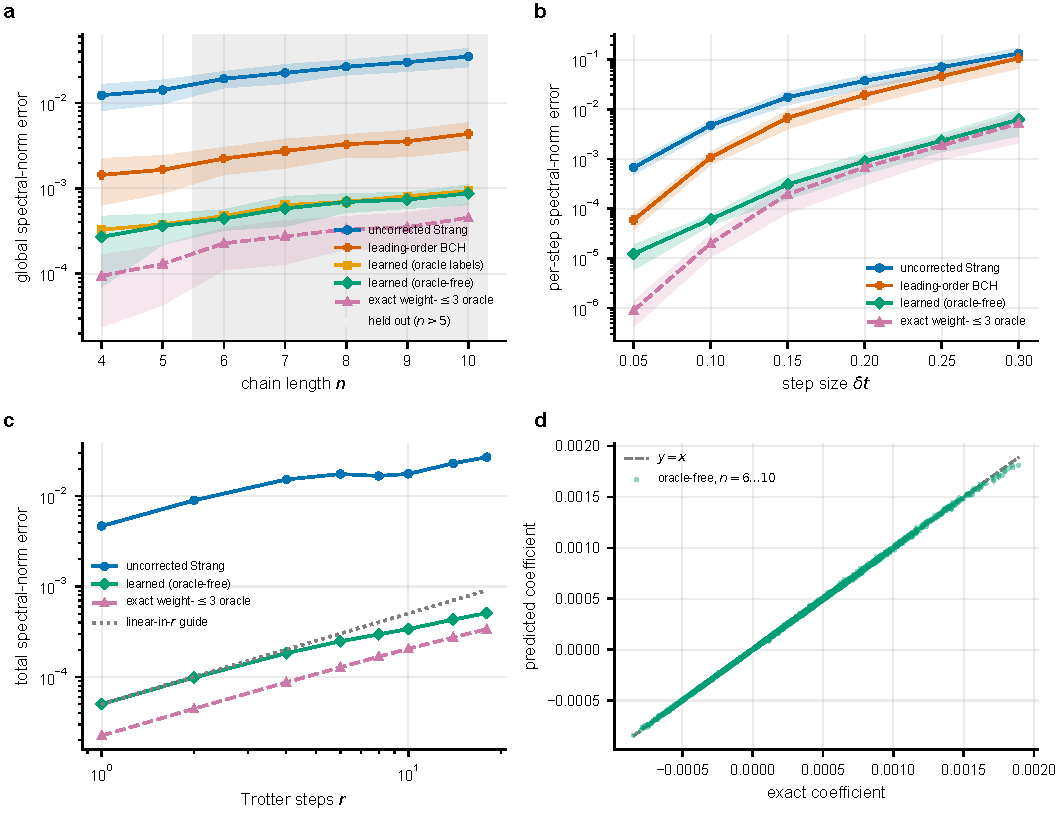
\includegraphics[width=\linewidth]{fig5_learned_transfer.pdf}
\caption{\textbf{Learned residual generators on the disordered \tfim{}.} Shaded bands are one standard deviation over disordered realizations. \textbf{a}, Global spectral-norm error at $t=1$, $\dt=0.1$ versus chain length for the uncorrected Strang step, leading-order BCH, the prior-free learned ablation, the learned correction (analytic second-order Zassenhaus prior plus learned residual) trained on oracle labels and on oracle-free patch labels (overlapping), and the exact weight-$\leq3$ oracle; the shaded region marks lengths absent from training ($n>5$), extending to $n=10$. \textbf{b}, Per-step error versus step size $\dt$ at $n=6$; leading-order BCH approaches the uncorrected step as $\dt$ grows, while the learned correction tracks the oracle. \textbf{c}, Total error versus number of Trotter steps $r$ ($n=6$, $\dt=0.1$), growing linearly in $r$ as Theorem~\ref{thm:residual-stability} predicts (grey guide). \textbf{d}, Oracle-free predicted versus exact coefficients on held-out transfer sizes $n=6,\dots,10$ ($R^2=0.9999$). One per-site network, trained only on $n=4,5$, sees only local couplings at inference.}
\label{fig:learned}
\end{figure}

\begin{table}[t]
\caption{\textbf{Learned residual generator transferred across system size on the disordered open-boundary \tfim{}.} Parameters are $J_i,h_i\sim\mathcal{U}[0.5,1.5]$, $t=1$, and $\dt=0.1$. Errors are global spectral-norm errors reported as the mean $\pm$ one standard deviation over the disordered chains (count $n_{\mathrm c}$ in the last column); the same dispersion is shown as bands in Fig.~\ref{fig:learned}. The column $\epsilon^{\mathrm{no\,prior}}_{\mathrm{learned}}$ is the ablation that learns the full generator directly; $\epsilon_{\mathrm{learned}}$ adds the analytic second-order Zassenhaus prior and learns only the residual beyond it. The reduction factor is $\epsilon_{\mathrm{Strang}}/\epsilon_{\mathrm{learned}}$. The oracle-free network is trained only on $n=4,5$; sizes $n\geq6$ are absent from training. All values are recomputed from dense matrices.}
\label{tab:learned-summary}
\centering
\resizebox{\linewidth}{!}{%
\begin{tabular}{ccccccc}
\toprule
$n$ & regime & $\epsilon_{\mathrm{Strang}}$ & $\epsilon^{\mathrm{no\,prior}}_{\mathrm{learned}}$ & $\epsilon_{\mathrm{learned}}$ & reduction & $n_{\mathrm c}$\\
\midrule
4 & train & $1.049\times10^{-2} \pm 3.269\times10^{-3}$ & $2.262\times10^{-4} \pm 9.235\times10^{-5}$ & $1.233\times10^{-4} \pm 4.460\times10^{-5}$ & $85.1\times$ & 40\\
5 & train & $1.549\times10^{-2} \pm 4.883\times10^{-3}$ & $3.557\times10^{-4} \pm 1.316\times10^{-4}$ & $2.176\times10^{-4} \pm 1.004\times10^{-4}$ & $71.2\times$ & 40\\
6 & transfer & $1.844\times10^{-2} \pm 4.841\times10^{-3}$ & $4.591\times10^{-4} \pm 1.725\times10^{-4}$ & $2.615\times10^{-4} \pm 9.708\times10^{-5}$ & $70.5\times$ & 40\\
7 & transfer & $2.028\times10^{-2} \pm 5.384\times10^{-3}$ & $5.542\times10^{-4} \pm 1.785\times10^{-4}$ & $3.075\times10^{-4} \pm 1.186\times10^{-4}$ & $65.9\times$ & 40\\
8 & transfer & $2.433\times10^{-2} \pm 5.566\times10^{-3}$ & $6.185\times10^{-4} \pm 1.524\times10^{-4}$ & $3.615\times10^{-4} \pm 1.138\times10^{-4}$ & $67.3\times$ & 24\\
9 & transfer & $3.207\times10^{-2} \pm 6.808\times10^{-3}$ & $8.160\times10^{-4} \pm 1.799\times10^{-4}$ & $5.560\times10^{-4} \pm 1.535\times10^{-4}$ & $57.7\times$ & 16\\
10 & transfer & $3.668\times10^{-2} \pm 6.553\times10^{-3}$ & $8.944\times10^{-4} \pm 2.201\times10^{-4}$ & $5.810\times10^{-4} \pm 1.939\times10^{-4}$ & $63.1\times$ & 12\\
\bottomrule
\end{tabular}}
\end{table}

Figure~\ref{fig:headline} summarizes the headline comparison: at the largest held-out transfer size the learned correction is nearly two orders of magnitude below the uncorrected Strang step and roughly an order of magnitude below leading-order BCH, and its error-reduction factor over the uncorrected baseline holds across every chain length, including the held-out transfer sizes.

\begin{figure}[t]
\centering
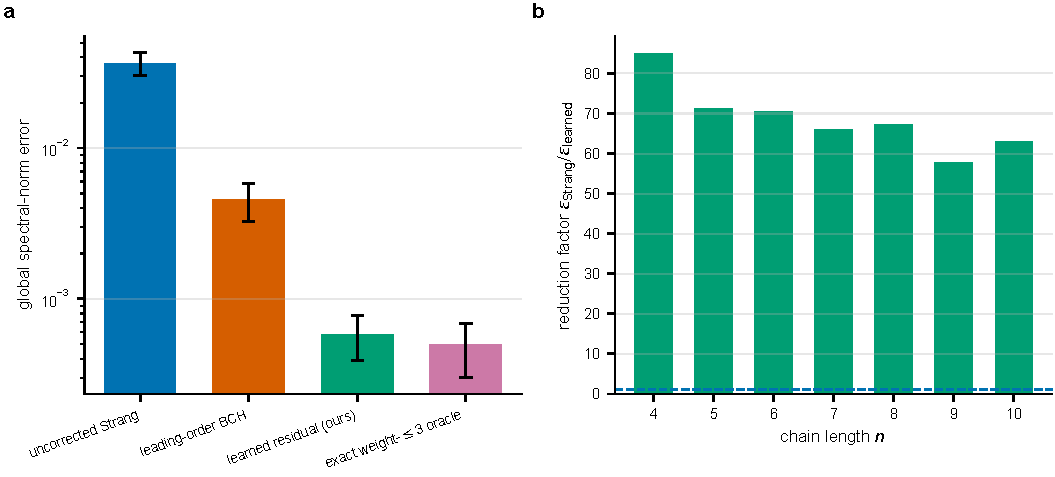
\includegraphics[width=\linewidth]{fig6_headline_improvement.pdf}
\caption{\textbf{Proposed learned correction versus all baselines.} \textbf{a}, Final global spectral-norm error at the largest held-out transfer size ($n=10$) for the uncorrected Strang step, leading-order BCH, the learned residual (ours), and the exact weight-$\leq3$ oracle; error bars show one standard deviation over disordered realizations. \textbf{b}, Error-reduction factor $\epsilon_{\mathrm{Strang}}/\epsilon_{\mathrm{learned}}$ of the learned correction over the uncorrected Strang baseline across all chain lengths, including the held-out transfer sizes $n\geq6$.}
\label{fig:headline}
\end{figure}

The per-step resource proxy separating baseline product-formula factors from dense oracle residual construction is given in Extended Data Table~\ref{tab:resources}. The residual matrix is not counted as a quantum gate; any practical implementation must replace dense residual construction by a compiled circuit, a local commutator formula, a learned generator, or another efficient representation.

% ============================================================
% DISCUSSION
% ============================================================

\section{Discussion}
\label{sec:discussion}

The exact residual identity alone is not a practical algorithm; its value is as the certified target of a chain of constructions that turn it into one. The framework combines: (i) a uniquely defined optimal correction target; (ii) stability theorems---shown order-optimal---that translate residual approximation error into global simulation error; (iii) a generator view exposing the defect as a small Hermitian operator; (iv) a spectral-truncation projection (Definition~\ref{def:spectral-truncation}) that makes compressed generators mathematically well posed with an \emph{a priori} certificate at every truncation level; (v) an order-generality locality theorem (Theorem~\ref{thm:order-locality}) showing the defect stays low-weight, hence compressible, at every order; (vi) a faithful-compilation theorem (Theorem~\ref{thm:faithful-compilation}) that converts the compressed generator into a counted two-qubit-gate circuit with a controlled error budget; (vii) the resulting error--cost frontier advance (Sec.~\ref{sec:frontier}); and (viii) a demonstration (Sec.~\ref{sec:learned}) that the generator can be \emph{learned} as a geometrically local, size-transferable operator inheriting the stability guarantee. This is a complete instance of ``oracle-to-algorithm'' research: many quantum algorithms begin with an ideal mathematical object and then build efficient block encodings, signal-processing polynomials, compilation methods, or randomized estimators around it~\cite{berry2015prl,low2017qsp,low2019qubitization,childs2022}. Here the ideal object is the residual generator, and the contribution is to compress it, compile it, learn it, and show that doing so moves the algorithm's accuracy--cost frontier.

\rgtc{} differs from existing strategies but is compatible with them. Multi-product formulas cancel leading Trotter errors by linearly combining unitaries~\cite{childs2012mpf}; randomized formulas reduce error in expectation or concentration~\cite{campbell2019,ouyang2020,childs2022,chen2022a}; qubitization and quantum signal processing implement polynomial transformations of block encodings~\cite{berry2007,berry2014,low2017qsp,low2019qubitization}; Magnus methods construct effective generators for time-dependent or interaction-picture dynamics~\cite{magnus1954,blanes2009,sharma2024,fang2025}. \rgtc{} keeps the product-formula step and corrects it by a residual generator, so one could define a residual for a randomized product-formula realization, a multi-product formula, or a low-depth Cartan-decomposition circuit~\cite{kokcu2022,steckmann2023}.

The projected residual experiment is the most important empirical component beyond the tautological oracle identity. In the dense \tfim{} benchmark at $n=5$, $q=2$, $t=1$, the baseline error is $1.384\times10^{-2}$; the $w\leq3$ projected generator reduces this to $1.545\times10^{-4}$, while $w\leq4$ reduces it to $1.850\times10^{-7}$. These are still dense offline experiments, but they demonstrate that most of the useful correction can live in a dramatically smaller operator family, and Theorem~\ref{thm:tfim-support} explains why weight three is the first meaningful threshold for the leading Strang defect in this regime.

Near-term quantum algorithms, including VQE~\cite{peruzzo2014,mcclean2016}, QAOA~\cite{farhi2014,huynh2026uqqaoa}, and broader variational workflows~\cite{cerezo2021,bharti2022,endo2021}, are constrained by circuit depth and noise~\cite{preskill2018,kandala2017,kim2023}. A shallow residual generator could be used as a correction layer after a product-formula block, but only if it can be compiled into native gates with tolerable overhead. Fault-tolerant settings shift the question toward T-count, block encodings, and resource estimates~\cite{wecker2014,wecker2015,babbush2018,babbush2019,haah2021}. In either regime, Theorem~\ref{thm:residual-stability} supplies a simple target: if a compiled residual has per-step operator error at most $\epsilon/r$, then the global simulation error contribution is at most $\epsilon$. The benchmark suite is dense-linear-algebra heavy and parameter-sweep heavy, hence naturally suited to GPU acceleration, which would enable larger offline training sets for learned residual generators and more serious benchmarking of compression families without changing the theory.

The limitations are real and we state them precisely, because the value of the frontier claim depends on not overstating it. \emph{First, the cost advantage is not uniform.} The correction's two-qubit-gate count grows slightly faster with $n$ than the next standard order, so the corrected fourth-order step is more accurate than sixth order at comparable cost but is not cheaper than sixth order; the genuine, robust statement (Sec.~\ref{sec:frontier}) is that it reaches a new accuracy regime---between consecutive standard orders---at $4.2$--$5.2\times$ fewer two-qubit gates than the cheapest standard formula attaining the same accuracy. \emph{Second, the compiled correction has an accuracy floor} set by the first-order inner product formula (Theorem~\ref{thm:faithful-compilation}); reaching below $\sim10^{-10}$ would require a second-order inner compilation, a direct extension we do not pursue here. \emph{Third, the oracle-free realization of the fourth-order frontier correction is only partly established.} On the positive side, that correction is built entirely from local weight-$\leq5$ templates and stays Pareto-optimal to $n=10$ (Table~\ref{tab:oracle-free-q4}), so by Theorem~\ref{thm:order-locality} it is in principle obtainable from a fixed, size-independent reference patch. But we verified that a small ($8$-qubit) patch is not yet bulk-converged for the $q=4$ generator---its tiled coefficients reach only $\sim10^{-7}$ at $n=10$, an order of magnitude above the direct local correction---so a fully oracle-free realization at frontier accuracy requires a larger size-independent patch or the learned per-site map demonstrated at second order (transferring to ten qubits). Verifying either at frontier accuracy needs a ${>}12$-qubit patch with a still-larger dense target, beyond our dense reach ($n\le10$); we report this honestly rather than overstate transfer. \emph{Fourth}, evaluation is by dense simulation up to ten qubits and the templates are model-specific; the XXZ results (Sec.~\ref{sec:xxz}) show the mechanism generalizes but with a larger, splitting-dependent weight threshold. The paper proves correction, compression, and compilation guarantees and exhibits a concrete frontier advance on benchmark spin chains; it does not claim a universal asymptotic quantum speedup. These limitations define the next tasks---second-order inner compilation, learned fourth-order corrections at scale, evaluation beyond dense simulation, and template families for broader Hamiltonians---each of which is implementation within the established principle rather than a change of it.

% ============================================================
% REFERENCES
% ============================================================

\begin{thebibliography}{10}
\expandafter\ifx\csname url\endcsname\relax
  \def\url#1{\texttt{#1}}\fi
\expandafter\ifx\csname urlprefix\endcsname\relax\def\urlprefix{URL }\fi
\providecommand{\bibinfo}[2]{#2}
\providecommand{\eprint}[2][]{\url{#2}}

\bibitem{lloyd1996}
\bibinfo{author}{Lloyd, S.}
\newblock \bibinfo{title}{Universal quantum simulators}.
\newblock \emph{\bibinfo{journal}{Science}} \textbf{\bibinfo{volume}{273}},
  \bibinfo{pages}{1073--1078} (\bibinfo{year}{1996}).

\bibitem{trotter1959}
\bibinfo{author}{Trotter, H.~F.}
\newblock \bibinfo{title}{On the product of semi-groups of operators}.
\newblock \emph{\bibinfo{journal}{Proceedings of the American Mathematical
  Society}} \textbf{\bibinfo{volume}{10}}, \bibinfo{pages}{545--551}
  (\bibinfo{year}{1959}).

\bibitem{suzuki1990}
\bibinfo{author}{Suzuki, M.}
\newblock \bibinfo{title}{Fractal decomposition of exponential operators with
  applications to many-body theories and {Monte Carlo} simulations}.
\newblock \emph{\bibinfo{journal}{Physics Letters A}}
  \textbf{\bibinfo{volume}{146}}, \bibinfo{pages}{319--323}
  (\bibinfo{year}{1990}).

\bibitem{suzuki1991}
\bibinfo{author}{Suzuki, M.}
\newblock \bibinfo{title}{General theory of fractal path integrals with
  applications to many-body theories and statistical physics}.
\newblock \emph{\bibinfo{journal}{Journal of Mathematical Physics}}
  \textbf{\bibinfo{volume}{32}}, \bibinfo{pages}{400--407}
  (\bibinfo{year}{1991}).

\bibitem{suzuki1993}
\bibinfo{author}{Suzuki, M.}
\newblock \bibinfo{title}{Improved {Trotter}-like formulae}.
\newblock \emph{\bibinfo{journal}{Journal of Physics A: Mathematical and
  General}} \textbf{\bibinfo{volume}{26}}, \bibinfo{pages}{L133--L137}
  (\bibinfo{year}{1993}).

\bibitem{yoshida1990}
\bibinfo{author}{Yoshida, H.}
\newblock \bibinfo{title}{Construction of higher order symplectic integrators}.
\newblock \emph{\bibinfo{journal}{Physics Letters A}}
  \textbf{\bibinfo{volume}{150}}, \bibinfo{pages}{262--268}
  (\bibinfo{year}{1990}).

\bibitem{forest1990}
\bibinfo{author}{Forest, E.} \& \bibinfo{author}{Ruth, R.~D.}
\newblock \bibinfo{title}{Fourth-order symplectic integration}.
\newblock \emph{\bibinfo{journal}{Physica D: Nonlinear Phenomena}}
  \textbf{\bibinfo{volume}{43}}, \bibinfo{pages}{105--117}
  (\bibinfo{year}{1990}).

\bibitem{chin1997}
\bibinfo{author}{Chin, S.~A.}
\newblock \bibinfo{title}{Symplectic integrators from composite operator
  factorizations}.
\newblock \emph{\bibinfo{journal}{Physics Letters A}}
  \textbf{\bibinfo{volume}{226}}, \bibinfo{pages}{344--348}
  (\bibinfo{year}{1997}).

\bibitem{hatano2005}
\bibinfo{author}{Hatano, N.} \& \bibinfo{author}{Suzuki, M.}
\newblock \bibinfo{title}{Finding exponential product formulas of higher
  orders}.
\newblock In \bibinfo{editor}{Das, A.} \& \bibinfo{editor}{Chakrabarti, B.~K.}
  (eds.) \emph{\bibinfo{booktitle}{Quantum Annealing and Other Optimization
  Methods}}, \bibinfo{pages}{37--68} (\bibinfo{publisher}{Springer},
  \bibinfo{address}{Berlin}, \bibinfo{year}{2005}).

\bibitem{wiebe2010}
\bibinfo{author}{Wiebe, N.}, \bibinfo{author}{Berry, D.},
  \bibinfo{author}{H{\o}yer, P.} \& \bibinfo{author}{Sanders, B.~C.}
\newblock \bibinfo{title}{Higher order decompositions of ordered operator
  exponentials}.
\newblock \emph{\bibinfo{journal}{Journal of Physics A: Mathematical and
  Theoretical}} \textbf{\bibinfo{volume}{43}}, \bibinfo{pages}{065203}
  (\bibinfo{year}{2010}).

\bibitem{abrams1997}
\bibinfo{author}{Abrams, D.~S.} \& \bibinfo{author}{Lloyd, S.}
\newblock \bibinfo{title}{Simulation of many-body {Fermi} systems on a
  universal quantum computer}.
\newblock \emph{\bibinfo{journal}{Physical Review Letters}}
  \textbf{\bibinfo{volume}{79}}, \bibinfo{pages}{2586--2589}
  (\bibinfo{year}{1997}).

\bibitem{sornborger1999}
\bibinfo{author}{Sornborger, A.~T.} \& \bibinfo{author}{Stewart, E.~D.}
\newblock \bibinfo{title}{Higher-order methods for simulations on quantum
  computers}.
\newblock \emph{\bibinfo{journal}{Physical Review A}}
  \textbf{\bibinfo{volume}{60}}, \bibinfo{pages}{1956--1965}
  (\bibinfo{year}{1999}).

\bibitem{ortiz2001}
\bibinfo{author}{Ortiz, G.}, \bibinfo{author}{Gubernatis, J.~E.},
  \bibinfo{author}{Knill, E.} \& \bibinfo{author}{Laflamme, R.}
\newblock \bibinfo{title}{Quantum algorithms for fermionic simulations}.
\newblock \emph{\bibinfo{journal}{Physical Review A}}
  \textbf{\bibinfo{volume}{64}}, \bibinfo{pages}{022319}
  (\bibinfo{year}{2001}).

\bibitem{kitaev1997}
\bibinfo{author}{Kitaev, A.~Y.}
\newblock \bibinfo{title}{Quantum computations: algorithms and error
  correction}.
\newblock \emph{\bibinfo{journal}{Russian Mathematical Surveys}}
  \textbf{\bibinfo{volume}{52}}, \bibinfo{pages}{1191--1249}
  (\bibinfo{year}{1997}).

\bibitem{kitaev2002}
\bibinfo{author}{Kitaev, A.~Y.}, \bibinfo{author}{Shen, A.~H.} \&
  \bibinfo{author}{Vyalyi, M.~N.}
\newblock \emph{\bibinfo{title}{Classical and Quantum Computation}}
  (\bibinfo{publisher}{American Mathematical Society},
  \bibinfo{address}{Providence, Rhode Island}, \bibinfo{year}{2002}).

\bibitem{abrams1999}
\bibinfo{author}{Abrams, D.~S.} \& \bibinfo{author}{Lloyd, S.}
\newblock \bibinfo{title}{Quantum algorithm providing exponential speed
  increase for finding eigenvalues and eigenvectors}.
\newblock \emph{\bibinfo{journal}{Physical Review Letters}}
  \textbf{\bibinfo{volume}{83}}, \bibinfo{pages}{5162--5165}
  (\bibinfo{year}{1999}).

\bibitem{cleve1998}
\bibinfo{author}{Cleve, R.}, \bibinfo{author}{Ekert, A.},
  \bibinfo{author}{Macchiavello, C.} \& \bibinfo{author}{Mosca, M.}
\newblock \bibinfo{title}{Quantum algorithms revisited}.
\newblock \emph{\bibinfo{journal}{Proceedings of the Royal Society of London,
  Series A}} \textbf{\bibinfo{volume}{454}}, \bibinfo{pages}{339--354}
  (\bibinfo{year}{1998}).

\bibitem{aspuruguzik2005}
\bibinfo{author}{Aspuru-Guzik, A.}, \bibinfo{author}{Dutoi, A.~D.},
  \bibinfo{author}{Love, P.~J.} \& \bibinfo{author}{Head-Gordon, M.}
\newblock \bibinfo{title}{Simulated quantum computation of molecular energies}.
\newblock \emph{\bibinfo{journal}{Science}} \textbf{\bibinfo{volume}{309}},
  \bibinfo{pages}{1704--1707} (\bibinfo{year}{2005}).

\bibitem{wecker2014}
\bibinfo{author}{Wecker, D.}, \bibinfo{author}{Bauer, B.},
  \bibinfo{author}{Clark, B.~K.}, \bibinfo{author}{Hastings, M.~B.} \&
  \bibinfo{author}{Troyer, M.}
\newblock \bibinfo{title}{Gate-count estimates for performing quantum chemistry
  on small quantum computers}.
\newblock \emph{\bibinfo{journal}{Physical Review A}}
  \textbf{\bibinfo{volume}{90}}, \bibinfo{pages}{022305}
  (\bibinfo{year}{2014}).

\bibitem{wecker2015}
\bibinfo{author}{Wecker, D.}, \bibinfo{author}{Bauer, B.},
  \bibinfo{author}{Clark, B.~K.}, \bibinfo{author}{Hastings, M.~B.} \&
  \bibinfo{author}{Troyer, M.}
\newblock \bibinfo{title}{Progress towards practical quantum advantage in
  quantum chemistry simulations}.
\newblock \emph{\bibinfo{journal}{Physical Review A}}
  \textbf{\bibinfo{volume}{92}}, \bibinfo{pages}{042303}
  (\bibinfo{year}{2015}).

\bibitem{babbush2015}
\bibinfo{author}{Babbush, R.}, \bibinfo{author}{McClean, J.},
  \bibinfo{author}{Wecker, D.}, \bibinfo{author}{Aspuru-Guzik, A.} \&
  \bibinfo{author}{Wiebe, N.}
\newblock \bibinfo{title}{Chemical basis of {Trotter}-{Suzuki} errors in
  quantum chemistry simulations}.
\newblock \emph{\bibinfo{journal}{Physical Review A}}
  \textbf{\bibinfo{volume}{91}}, \bibinfo{pages}{022311}
  (\bibinfo{year}{2015}).

\bibitem{reiher2017}
\bibinfo{author}{Reiher, M.}, \bibinfo{author}{Wiebe, N.},
  \bibinfo{author}{Svore, K.~M.}, \bibinfo{author}{Wecker, D.} \&
  \bibinfo{author}{Troyer, M.}
\newblock \bibinfo{title}{Elucidating reaction mechanisms on quantum
  computers}.
\newblock \emph{\bibinfo{journal}{Proceedings of the National Academy of
  Sciences}} \textbf{\bibinfo{volume}{114}}, \bibinfo{pages}{7555--7560}
  (\bibinfo{year}{2017}).

\bibitem{kivlichan2018}
\bibinfo{author}{Kivlichan, I.~D.} \emph{et~al.}
\newblock \bibinfo{title}{Quantum simulation of electronic structure with
  linear depth and connectivity}.
\newblock \emph{\bibinfo{journal}{Physical Review Letters}}
  \textbf{\bibinfo{volume}{120}}, \bibinfo{pages}{110501}
  (\bibinfo{year}{2018}).

\bibitem{haah2021}
\bibinfo{author}{Haah, J.}, \bibinfo{author}{Hastings, M.~B.},
  \bibinfo{author}{Kothari, R.} \& \bibinfo{author}{Low, G.~H.}
\newblock \bibinfo{title}{Quantum algorithm for simulating real time dynamics
  of lattice {Hamiltonians}}.
\newblock \emph{\bibinfo{journal}{SIAM Journal on Computing}}
  \textbf{\bibinfo{volume}{52}}, \bibinfo{pages}{1534--1565}
  (\bibinfo{year}{2021}).
\newblock \eprint{1801.00862}.

\bibitem{childs2021}
\bibinfo{author}{Childs, A.~M.}, \bibinfo{author}{Su, Y.},
  \bibinfo{author}{Tran, M.~C.}, \bibinfo{author}{Wiebe, N.} \&
  \bibinfo{author}{Zhu, S.}
\newblock \bibinfo{title}{Theory of {Trotter} error with commutator scaling}.
\newblock \emph{\bibinfo{journal}{PRX Quantum}} \textbf{\bibinfo{volume}{2}},
  \bibinfo{pages}{010329} (\bibinfo{year}{2021}).

\bibitem{layden2022}
\bibinfo{author}{Layden, D.}
\newblock \bibinfo{title}{First-order {Trotter} error from a second-order
  perspective}.
\newblock \emph{\bibinfo{journal}{Physical Review Letters}}
  \textbf{\bibinfo{volume}{128}}, \bibinfo{pages}{210501}
  (\bibinfo{year}{2022}).

\bibitem{zhuk2023}
\bibinfo{author}{Zhuk, S.}, \bibinfo{author}{Sun, N.~F.} \&
  \bibinfo{author}{Bravyi, S.}
\newblock \bibinfo{title}{{Trotter} error bounds and dynamic structure factors
  for quantum spin systems far from equilibrium}.
\newblock \emph{\bibinfo{journal}{PRX Quantum}} \textbf{\bibinfo{volume}{4}},
  \bibinfo{pages}{020345} (\bibinfo{year}{2023}).

\bibitem{childs2019lattice}
\bibinfo{author}{Childs, A.~M.} \& \bibinfo{author}{Su, Y.}
\newblock \bibinfo{title}{Nearly optimal lattice simulation by product
  formulas}.
\newblock \emph{\bibinfo{journal}{Physical Review Letters}}
  \textbf{\bibinfo{volume}{123}}, \bibinfo{pages}{050503}
  (\bibinfo{year}{2019}).

\bibitem{lieb1972}
\bibinfo{author}{Lieb, E.~H.} \& \bibinfo{author}{Robinson, D.~W.}
\newblock \bibinfo{title}{The finite group velocity of quantum spin systems}.
\newblock \emph{\bibinfo{journal}{Communications in Mathematical Physics}}
  \textbf{\bibinfo{volume}{28}}, \bibinfo{pages}{251--257}
  (\bibinfo{year}{1972}).

\bibitem{tran2020}
\bibinfo{author}{Tran, M.~C.} \emph{et~al.}
\newblock \bibinfo{title}{Locality and digital quantum simulation of power-law
  interactions}.
\newblock \emph{\bibinfo{journal}{Physical Review X}}
  \textbf{\bibinfo{volume}{9}}, \bibinfo{pages}{031006} (\bibinfo{year}{2019}).

\bibitem{low2023pra}
\bibinfo{author}{Low, G.~H.}, \bibinfo{author}{Su, Y.}, \bibinfo{author}{Tong,
  Y.} \& \bibinfo{author}{Tran, M.~C.}
\newblock \bibinfo{title}{Complexity of implementing {Trotter} steps}.
\newblock \emph{\bibinfo{journal}{PRX Quantum}} \textbf{\bibinfo{volume}{4}},
  \bibinfo{pages}{020323} (\bibinfo{year}{2023}).

\bibitem{childs2012mpf}
\bibinfo{author}{Childs, A.~M.} \& \bibinfo{author}{Wiebe, N.}
\newblock \bibinfo{title}{Hamiltonian simulation using linear combinations of
  unitary operations}.
\newblock \emph{\bibinfo{journal}{Quantum Information \& Computation}}
  \textbf{\bibinfo{volume}{12}}, \bibinfo{pages}{901--924}
  (\bibinfo{year}{2012}).
\newblock \eprint{1202.5822}.

\bibitem{berry2015prl}
\bibinfo{author}{Berry, D.~W.}, \bibinfo{author}{Childs, A.~M.},
  \bibinfo{author}{Cleve, R.}, \bibinfo{author}{Kothari, R.} \&
  \bibinfo{author}{Somma, R.~D.}
\newblock \bibinfo{title}{Simulating hamiltonian dynamics with a truncated
  {Taylor} series}.
\newblock \emph{\bibinfo{journal}{Physical Review Letters}}
  \textbf{\bibinfo{volume}{114}}, \bibinfo{pages}{090502}
  (\bibinfo{year}{2015}).

\bibitem{berry2007}
\bibinfo{author}{Berry, D.~W.}, \bibinfo{author}{Ahokas, G.},
  \bibinfo{author}{Cleve, R.} \& \bibinfo{author}{Sanders, B.~C.}
\newblock \bibinfo{title}{Efficient quantum algorithms for simulating sparse
  {Hamiltonians}}.
\newblock \emph{\bibinfo{journal}{Communications in Mathematical Physics}}
  \textbf{\bibinfo{volume}{270}}, \bibinfo{pages}{359--371}
  (\bibinfo{year}{2007}).

\bibitem{berry2014}
\bibinfo{author}{Berry, D.~W.}, \bibinfo{author}{Childs, A.~M.},
  \bibinfo{author}{Cleve, R.}, \bibinfo{author}{Kothari, R.} \&
  \bibinfo{author}{Somma, R.~D.}
\newblock \bibinfo{title}{Exponential improvement in precision for simulating
  sparse {Hamiltonians} via quantum walks}.
\newblock In \emph{\bibinfo{booktitle}{Proceedings of the 46th Annual ACM
  Symposium on Theory of Computing}}, \bibinfo{pages}{283--292}
  (\bibinfo{year}{2014}).

\bibitem{low2017qsp}
\bibinfo{author}{Low, G.~H.} \& \bibinfo{author}{Chuang, I.~L.}
\newblock \bibinfo{title}{Optimal {Hamiltonian} simulation by quantum signal
  processing}.
\newblock \emph{\bibinfo{journal}{Physical Review Letters}}
  \textbf{\bibinfo{volume}{118}}, \bibinfo{pages}{010501}
  (\bibinfo{year}{2017}).

\bibitem{low2019qubitization}
\bibinfo{author}{Low, G.~H.} \& \bibinfo{author}{Chuang, I.~L.}
\newblock \bibinfo{title}{Hamiltonian simulation by qubitization}.
\newblock \emph{\bibinfo{journal}{Quantum}} \textbf{\bibinfo{volume}{3}},
  \bibinfo{pages}{163} (\bibinfo{year}{2019}).

\bibitem{campbell2019}
\bibinfo{author}{Campbell, E.~T.}
\newblock \bibinfo{title}{Random compiler for fast {Hamiltonian} simulation}.
\newblock \emph{\bibinfo{journal}{Physical Review Letters}}
  \textbf{\bibinfo{volume}{123}}, \bibinfo{pages}{070503}
  (\bibinfo{year}{2019}).

\bibitem{ouyang2020}
\bibinfo{author}{Ouyang, Y.}, \bibinfo{author}{White, D.~R.} \&
  \bibinfo{author}{Campbell, E.~T.}
\newblock \bibinfo{title}{Compilation by stochastic {Hamiltonian}
  sparsification}.
\newblock \emph{\bibinfo{journal}{Quantum}} \textbf{\bibinfo{volume}{4}},
  \bibinfo{pages}{235} (\bibinfo{year}{2020}).

\bibitem{childs2022}
\bibinfo{author}{Childs, A.~M.}, \bibinfo{author}{Ostrander, A.} \&
  \bibinfo{author}{Su, Y.}
\newblock \bibinfo{title}{Faster quantum simulation by randomization}.
\newblock \emph{\bibinfo{journal}{Quantum}} \textbf{\bibinfo{volume}{3}},
  \bibinfo{pages}{182} (\bibinfo{year}{2019}).

\bibitem{chen2022a}
\bibinfo{author}{Chen, C.-F.}, \bibinfo{author}{Huang, H.-Y.},
  \bibinfo{author}{Kueng, R.} \& \bibinfo{author}{Tropp, J.~A.}
\newblock \bibinfo{title}{Concentration for random product formulas}.
\newblock \emph{\bibinfo{journal}{PRX Quantum}} \textbf{\bibinfo{volume}{2}},
  \bibinfo{pages}{040305} (\bibinfo{year}{2021}).

\bibitem{magnus1954}
\bibinfo{author}{Magnus, W.}
\newblock \bibinfo{title}{On the exponential solution of differential equations
  for a linear operator}.
\newblock \emph{\bibinfo{journal}{Communications on Pure and Applied
  Mathematics}} \textbf{\bibinfo{volume}{7}}, \bibinfo{pages}{649--673}
  (\bibinfo{year}{1954}).

\bibitem{blanes2009}
\bibinfo{author}{Blanes, S.}, \bibinfo{author}{Casas, F.},
  \bibinfo{author}{Oteo, J.~A.} \& \bibinfo{author}{Ros, J.}
\newblock \bibinfo{title}{The {Magnus} expansion and some of its applications}.
\newblock \emph{\bibinfo{journal}{Physics Reports}}
  \textbf{\bibinfo{volume}{470}}, \bibinfo{pages}{151--238}
  (\bibinfo{year}{2009}).

\bibitem{sharma2024}
\bibinfo{author}{Sharma, K.} \& \bibinfo{author}{Tran, M.~C.}
\newblock \bibinfo{title}{Hamiltonian simulation in the interaction picture
  using the {Magnus} expansion}.
\newblock \emph{\bibinfo{journal}{Physical Review Research}}
  \textbf{\bibinfo{volume}{6}}, \bibinfo{pages}{033047} (\bibinfo{year}{2024}).

\bibitem{fang2025}
\bibinfo{author}{Fang, D.}, \bibinfo{author}{Liu, D.} \&
  \bibinfo{author}{Sarkar, R.}
\newblock \bibinfo{title}{Time-dependent hamiltonian simulation via {Magnus}
  expansion: Algorithm and superconvergence}.
\newblock \emph{\bibinfo{journal}{Communications in Mathematical Physics}}
  \textbf{\bibinfo{volume}{406}}, \bibinfo{pages}{128} (\bibinfo{year}{2025}).

\bibitem{cirstoiu2020}
\bibinfo{author}{Cirstoiu, C.} \emph{et~al.}
\newblock \bibinfo{title}{Variational fast forwarding for quantum simulation
  beyond the coherence time}.
\newblock \emph{\bibinfo{journal}{npj Quantum Information}}
  \textbf{\bibinfo{volume}{6}}, \bibinfo{pages}{82} (\bibinfo{year}{2020}).

\bibitem{kokcu2022}
\bibinfo{author}{Kökçü, E.} \emph{et~al.}
\newblock \bibinfo{title}{Fixed depth hamiltonian simulation via {Cartan}
  decomposition}.
\newblock \emph{\bibinfo{journal}{Physical Review Letters}}
  \textbf{\bibinfo{volume}{129}}, \bibinfo{pages}{070501}
  (\bibinfo{year}{2022}).

\bibitem{steckmann2023}
\bibinfo{author}{Steckmann, T.} \emph{et~al.}
\newblock \bibinfo{title}{Simulating the {Mott} transition on a noisy digital
  quantum computer via {Cartan}-based fast-forwarding circuits}.
\newblock \emph{\bibinfo{journal}{PRX Quantum}} \textbf{\bibinfo{volume}{4}},
  \bibinfo{pages}{010308} (\bibinfo{year}{2023}).

\bibitem{wu2023}
\bibinfo{author}{Wu, S.-X.}, \bibinfo{author}{Du, S.-W.},
  \bibinfo{author}{Fang, D.} \& \bibinfo{author}{Liu, D.-S.}
\newblock \bibinfo{title}{Randomized hamiltonian simulation by magnetic
  groups}.
\newblock \emph{\bibinfo{journal}{Physical Review A}}
  \textbf{\bibinfo{volume}{108}}, \bibinfo{pages}{022418}
  (\bibinfo{year}{2023}).

\bibitem{zeier2011}
\bibinfo{author}{Zeier, R.} \& \bibinfo{author}{Schulte-Herbr\"{u}ggen, T.}
\newblock \bibinfo{title}{Symmetry principles in quantum systems theory}.
\newblock \emph{\bibinfo{journal}{Journal of Mathematical Physics}}
  \textbf{\bibinfo{volume}{52}}, \bibinfo{pages}{113510}
  (\bibinfo{year}{2011}).

\bibitem{sachdev2011}
\bibinfo{author}{Sachdev, S.}
\newblock \emph{\bibinfo{title}{Quantum Phase Transitions}}
  (\bibinfo{publisher}{Cambridge University Press},
  \bibinfo{address}{Cambridge}, \bibinfo{year}{2011}), \bibinfo{edition}{2nd}
  edn.

\bibitem{cerveralierta2018}
\bibinfo{author}{Cervera-Lierta, A.}
\newblock \bibinfo{title}{Exact {Ising} model simulation on a quantum
  computer}.
\newblock \emph{\bibinfo{journal}{Quantum}} \textbf{\bibinfo{volume}{2}},
  \bibinfo{pages}{114} (\bibinfo{year}{2018}).

\bibitem{bravyi2002}
\bibinfo{author}{Bravyi, S.~B.} \& \bibinfo{author}{Kitaev, A.~Y.}
\newblock \bibinfo{title}{Fermionic quantum computation}.
\newblock \emph{\bibinfo{journal}{Annals of Physics}}
  \textbf{\bibinfo{volume}{298}}, \bibinfo{pages}{210--226}
  (\bibinfo{year}{2002}).

\bibitem{whitfield2011}
\bibinfo{author}{Whitfield, J.~D.}, \bibinfo{author}{Biamonte, J.} \&
  \bibinfo{author}{Aspuru-Guzik, A.}
\newblock \bibinfo{title}{Simulation of electronic structure {Hamiltonians}
  using quantum computers}.
\newblock \emph{\bibinfo{journal}{Molecular Physics}}
  \textbf{\bibinfo{volume}{109}}, \bibinfo{pages}{735--750}
  (\bibinfo{year}{2011}).

\bibitem{seeley2012}
\bibinfo{author}{Seeley, J.~T.}, \bibinfo{author}{Richard, M.~J.} \&
  \bibinfo{author}{Love, P.~J.}
\newblock \bibinfo{title}{The {Bravyi}-{Kitaev} transformation for quantum
  computation of electronic structure}.
\newblock \emph{\bibinfo{journal}{Journal of Chemical Physics}}
  \textbf{\bibinfo{volume}{137}}, \bibinfo{pages}{224109}
  (\bibinfo{year}{2012}).

\bibitem{verstraete2005}
\bibinfo{author}{Verstraete, F.} \& \bibinfo{author}{Cirac, J.~I.}
\newblock \bibinfo{title}{Mapping local {Hamiltonians} of fermions to local
  {Hamiltonians} of spins}.
\newblock \emph{\bibinfo{journal}{Journal of Statistical Mechanics: Theory and
  Experiment}} \textbf{\bibinfo{volume}{2005}}, \bibinfo{pages}{P09012}
  (\bibinfo{year}{2005}).

\bibitem{cade2020}
\bibinfo{author}{Cade, C.}, \bibinfo{author}{Mineh, L.},
  \bibinfo{author}{Montanaro, A.} \& \bibinfo{author}{Sherborn, S.}
\newblock \bibinfo{title}{Strategies for solving the {Fermi-Hubbard} model on
  near-term quantum computers}.
\newblock \emph{\bibinfo{journal}{Physical Review B}}
  \textbf{\bibinfo{volume}{102}}, \bibinfo{pages}{235122}
  (\bibinfo{year}{2020}).

\bibitem{jordan2012}
\bibinfo{author}{Jordan, S.~P.}, \bibinfo{author}{Lee, K. S.~M.} \&
  \bibinfo{author}{Preskill, J.}
\newblock \bibinfo{title}{Quantum algorithms for quantum field theories}.
\newblock \emph{\bibinfo{journal}{Science}} \textbf{\bibinfo{volume}{336}},
  \bibinfo{pages}{1130--1133} (\bibinfo{year}{2012}).

\bibitem{babbush2018}
\bibinfo{author}{Babbush, R.} \emph{et~al.}
\newblock \bibinfo{title}{Encoding electronic spectra in quantum circuits with
  linear {T} complexity}.
\newblock \emph{\bibinfo{journal}{Physical Review X}}
  \textbf{\bibinfo{volume}{8}}, \bibinfo{pages}{041015} (\bibinfo{year}{2018}).

\bibitem{babbush2019}
\bibinfo{author}{Babbush, R.}, \bibinfo{author}{Berry, D.~W.},
  \bibinfo{author}{McClean, J.~R.} \& \bibinfo{author}{Neven, H.}
\newblock \bibinfo{title}{Quantum simulation of chemistry with sublinear
  scaling in basis size}.
\newblock \emph{\bibinfo{journal}{npj Quantum Information}}
  \textbf{\bibinfo{volume}{5}}, \bibinfo{pages}{92} (\bibinfo{year}{2019}).

\bibitem{peruzzo2014}
\bibinfo{author}{Peruzzo, A.} \emph{et~al.}
\newblock \bibinfo{title}{A variational eigenvalue solver on a photonic chip}.
\newblock \emph{\bibinfo{journal}{Nature Communications}}
  \textbf{\bibinfo{volume}{5}}, \bibinfo{pages}{4213} (\bibinfo{year}{2014}).

\bibitem{mcclean2016}
\bibinfo{author}{McClean, J.~R.}, \bibinfo{author}{Romero, J.},
  \bibinfo{author}{Babbush, R.} \& \bibinfo{author}{Aspuru-Guzik, A.}
\newblock \bibinfo{title}{The theory of variational hybrid quantum-classical
  algorithms}.
\newblock \emph{\bibinfo{journal}{New Journal of Physics}}
  \textbf{\bibinfo{volume}{18}}, \bibinfo{pages}{023023}
  (\bibinfo{year}{2016}).

\bibitem{farhi2014}
\bibinfo{author}{Farhi, E.}, \bibinfo{author}{Goldstone, J.} \&
  \bibinfo{author}{Gutmann, S.}
\newblock \bibinfo{title}{A quantum approximate optimization algorithm}
  (\bibinfo{year}{2014}).
\newblock \eprint{1411.4028}.

\bibitem{cerezo2021}
\bibinfo{author}{Cerezo, M.} \emph{et~al.}
\newblock \bibinfo{title}{Variational quantum algorithms}.
\newblock \emph{\bibinfo{journal}{Nature Reviews Physics}}
  \textbf{\bibinfo{volume}{3}}, \bibinfo{pages}{625--644}
  (\bibinfo{year}{2021}).

\bibitem{bharti2022}
\bibinfo{author}{Bharti, K.} \emph{et~al.}
\newblock \bibinfo{title}{Noisy intermediate-scale quantum algorithms}.
\newblock \emph{\bibinfo{journal}{Reviews of Modern Physics}}
  \textbf{\bibinfo{volume}{94}}, \bibinfo{pages}{015004}
  (\bibinfo{year}{2022}).

\bibitem{endo2021}
\bibinfo{author}{Endo, S.}, \bibinfo{author}{Cai, Z.},
  \bibinfo{author}{Benjamin, S.~C.} \& \bibinfo{author}{Yuan, X.}
\newblock \bibinfo{title}{Hybrid quantum-classical algorithms and quantum error
  mitigation}.
\newblock \emph{\bibinfo{journal}{Journal of the Physical Society of Japan}}
  \textbf{\bibinfo{volume}{90}}, \bibinfo{pages}{032001}
  (\bibinfo{year}{2021}).

\bibitem{preskill2018}
\bibinfo{author}{Preskill, J.}
\newblock \bibinfo{title}{Quantum computing in the {NISQ} era and beyond}.
\newblock \emph{\bibinfo{journal}{Quantum}} \textbf{\bibinfo{volume}{2}},
  \bibinfo{pages}{79} (\bibinfo{year}{2018}).

\bibitem{kandala2017}
\bibinfo{author}{Kandala, A.} \emph{et~al.}
\newblock \bibinfo{title}{Hardware-efficient variational quantum eigensolver
  for small molecules and quantum magnets}.
\newblock \emph{\bibinfo{journal}{Nature}} \textbf{\bibinfo{volume}{549}},
  \bibinfo{pages}{242--246} (\bibinfo{year}{2017}).

\bibitem{kim2023}
\bibinfo{author}{Kim, Y.} \emph{et~al.}
\newblock \bibinfo{title}{Evidence for the utility of quantum computing before
  fault tolerance}.
\newblock \emph{\bibinfo{journal}{Nature}} \textbf{\bibinfo{volume}{618}},
  \bibinfo{pages}{500--505} (\bibinfo{year}{2023}).

\bibitem{huynh2026uqqaoa}
\bibinfo{author}{Huynh, M.}
\newblock \bibinfo{title}{Query-efficient quantum approximate optimization via graph-conditioned trust regions}.
\newblock \emph{\bibinfo{journal}{arXiv preprint arXiv:2604.24803}}
  (\bibinfo{year}{2026}).

\bibitem{nguyen2025zassenhaus}
\bibinfo{author}{Nguyen, M.} \& \bibinfo{author}{Jing, N.}
\newblock \bibinfo{title}{Zassenhaus expansion in solving the
  {Schr\"odinger} equation}.
\newblock \emph{\bibinfo{journal}{arXiv preprint arXiv:2505.09441}}
  (\bibinfo{year}{2025}).

\bibitem{jing2026complexity}
\bibinfo{author}{Jing, N.} \& \bibinfo{author}{Nguyen, M.}
\newblock \bibinfo{title}{Complexity bounds for {Hamiltonian} simulation in
  unitary representations}.
\newblock \emph{\bibinfo{journal}{arXiv preprint arXiv:2603.07231}}
  (\bibinfo{year}{2026}).

\bibitem{hashimoto2024spectral}
\bibinfo{author}{Hashimoto, Y.}, \bibinfo{author}{Hafid, A.},
  \bibinfo{author}{Ikeda, M.} \& \bibinfo{author}{Kadri, H.}
\newblock \bibinfo{title}{Spectral truncation kernels: noncommutativity in
  {$C^*$}-algebraic kernel machines}.
\newblock \emph{\bibinfo{journal}{Journal of Machine Learning Research}}
  (\bibinfo{year}{2024}).
\newblock \eprint{2405.17823}.

\bibitem{hashimoto2023rkhm}
\bibinfo{author}{Hashimoto, Y.}, \bibinfo{author}{Ikeda, M.} \&
  \bibinfo{author}{Kadri, H.}
\newblock \bibinfo{title}{Learning in {RKHM}: a {$C^*$}-algebraic twist for
  kernel machines}.
\newblock In \emph{\bibinfo{booktitle}{Proceedings of the 26th International
  Conference on Artificial Intelligence and Statistics (AISTATS)}}
  (\bibinfo{year}{2023}).

\end{thebibliography}

% ============================================================
% METHODS
% ============================================================

\section{Methods}
\label{sec:methods}

\subsection{Trotter--Suzuki steps and residual construction}

For $k\geq2$, higher even orders are generated by the Suzuki recursion
\begin{equation}
    S_{2k}(\dt)=S_{2k-2}(p_k\dt)^2S_{2k-2}((1-4p_k)\dt)S_{2k-2}(p_k\dt)^2,
    \qquad
    p_k=\left(4-4^{1/(2k-1)}\right)^{-1}.
    \label{eq:suzuki-recursion}
\end{equation}
For a fixed order $q$ and step size $\dt$, the residual factor is $R_q(\dt)=U(\dt)S_q(\dt)^\dagger$, the corrected one-step propagator is $G_q(\dt)=R_q(\dt)S_q(\dt)$, and the global approximation is $\widetilde U_{R,q}(t;r)=G_q(t/r)^r$. When $R_q$ is computed exactly, $G_q(\dt)=U(\dt)$. Because $R_q$ is unitary, it is represented as $R_q(\dt)=e^{-iK_q(\dt)}$ for a Hermitian residual generator $K_q$. The generator is not unique globally because eigenphases are defined modulo $2\pi$; for small enough $\dt$ the residual lies close to the identity and the principal generator is well defined.

A compressed residual generator is $\widehat K_q(\dt)\in\cB$, where $\cB\subseteq\mathsf{Herm}(d)$ is a real linear space of implementable Hermitian generators (Pauli strings of weight at most $w$, geometrically local Pauli strings of bounded diameter, commutator monomials up to a fixed degree, or generators representable by a fixed hardware ansatz), with $\widehat R_q(\dt)=e^{-i\widehat K_q(\dt)}$ and $\widehat G_q(\dt)=\widehat R_q(\dt)S_q(\dt)$. The most direct dense benchmark instantiation is Pauli projection. With $\cP_n=\{I,X,Y,Z\}^{\otimes n}$ and $\cB_w=\Span_\mathbb{R}\{P\in\cP_n:\operatorname{wt}(P)\leq w\}$, the projection is
\begin{equation}
    \Pi_wK_q=\sum_{\operatorname{wt}(P)\leq w}\frac{\Tr(PK_q)}{2^n}P.
    \label{eq:pauli-proj}
\end{equation}

\subsection{Theory: proofs}
\label{sec:theory}

This section contains the main mathematical guarantees. All norms are spectral norms unless explicitly stated otherwise.

\begin{lemma}[Unitarity of product-formula steps]
\label{lem:Sq-unitary}
Let $A$ and $B$ be Hermitian and let every Suzuki coefficient be real. Then $S_q(\dt)$ is unitary for every real $\dt$ and every $q\in\{1,2,4,6,8\}$ generated by the Strang step and Eq.~\eqref{eq:suzuki-recursion}.
\end{lemma}

\begin{proof}
Each elementary factor has the form $e^{-iC\tau}$ with $C=C^\dagger$ and $\tau\in\mathbb{R}$. Such a factor is unitary because $(e^{-iC\tau})^\dagger=e^{iC\tau}=(e^{-iC\tau})^{-1}$. The product of finitely many unitary matrices is unitary. The recursive Suzuki construction only composes such factors with real rescaled times, including the negative coefficient $1-4p_k$, which still gives a unitary exponential.
\end{proof}

\begin{theorem}[Exact residual factorization and uniqueness]
\label{thm:factorization}
Let $H=H^\dagger$ and let $S_q(\dt)$ be any unitary product-formula step. The residual $R_q(\dt)=U(\dt)S_q(\dt)^\dagger$ is unitary and is the unique matrix $L$ satisfying $LS_q(\dt)=U(\dt)$. Consequently, $R_q(\dt)S_q(\dt)=U(\dt)$ and $[R_q(t/r)S_q(t/r)]^r=U(t)$ for time-independent $H$.
\end{theorem}

\begin{proof}
Since $H$ is Hermitian, $U(\dt)$ is unitary. Lemma~\ref{lem:Sq-unitary} gives unitarity of $S_q$, hence $S_q^\dagger=S_q^{-1}$. Thus $R_q^\dagger R_q=S_qU^\dagger US_q^\dagger=S_qS_q^\dagger=\id$. Moreover, $R_qS_q=U S_q^\dagger S_q=U$. If $L S_q=U$, right multiplication by $S_q^\dagger$ gives $L=US_q^\dagger=R_q$. For $t=r\dt$, time independence gives $U(\dt)^r=U(r\dt)=U(t)$.
\end{proof}

\begin{theorem}[Optimality among all left corrections]
\label{thm:optimality}
Let $|||\cdot|||$ be any unitarily invariant norm. The residual $R_q$ is a global minimizer of $\mathcal{J}(L)=|||U(\dt)-LS_q(\dt)|||$. The minimum value is zero, and the minimizer is unique.
\end{theorem}

\begin{proof}
Every norm is nonnegative, so $\mathcal{J}(L)\geq0$. Theorem~\ref{thm:factorization} gives $\mathcal{J}(R_q)=0$. If another $L'$ also gives zero, then $L'S_q=U$, and uniqueness in Theorem~\ref{thm:factorization} implies $L'=R_q$.
\end{proof}

\begin{remark}
Theorem~\ref{thm:optimality} is an oracle statement, not a cost statement. It says that no exact left multiplier can beat $R_q$ in error because the error is already zero. It does not say that $R_q$ is cheap to implement.
\end{remark}

\begin{theorem}[Small-step residual-generator bound]
\label{thm:small-step}
Assume $S_q$ is order $q$ in the sense that there exist constants $C_q$ and $\dt_0$ such that $\norm{U(\dt)-S_q(\dt)}_2\leq C_q\abs{\dt}^{q+1}$ for $\abs{\dt}\leq\dt_0$. If $C_q\abs{\dt}^{q+1}\leq1$, then $R_q(\dt)$ has a Hermitian logarithm $K_q(\dt)$ with phases chosen in $[-\pi,\pi]$ and $\norm{K_q(\dt)}_2\leq 2C_q\abs{\dt}^{q+1}$.
\end{theorem}

\begin{proof}
Because $S_q$ is unitary, $\norm{R_q-\id}_2=\norm{US_q^\dagger-\id}_2=\norm{U-S_q}_2\leq C_q\abs{\dt}^{q+1}$. Diagonalize $R_q=W\operatorname{diag}(e^{-i\theta_j})W^\dagger$ with $\theta_j\in[-\pi,\pi]$ and define $K_q=W\operatorname{diag}(\theta_j)W^\dagger$. For any eigenphase, $\abs{e^{-i\theta_j}-1}=2\abs{\sin(\theta_j/2)}$. If $\norm{R_q-\id}_2\leq1$, then $\abs{\theta_j}\leq2\arcsin(\norm{R_q-\id}_2/2)\leq2\norm{R_q-\id}_2$. Taking the maximum over $j$ proves the bound.
\end{proof}

\begin{theorem}[Multi-step stability for approximate residuals]
\label{thm:residual-stability}
Let $\widehat R_q$ be any approximate residual and define $\widehat G_q=\widehat R_qS_q$. If $\eta=\norm{\widehat R_q-R_q}_2$, then
\begin{equation}
    \norm{\widehat G_q^{\;r}-U(t)}_2
    \leq \eta\sum_{j=0}^{r-1}(1+\eta)^j
    \leq r\eta e^{(r-1)\eta}.
    \label{eq:nonunitary-stability}
\end{equation}
If $\widehat R_q$ is unitary, then the sharper bound $\norm{\widehat G_q^{\;r}-U(t)}_2\leq r\eta$ holds.
\end{theorem}

\begin{proof}
Since $S_q$ is unitary, $\norm{\widehat G_q-G_q}_2=\norm{(\widehat R_q-R_q)S_q}_2=\eta$. Also $G_q=U(\dt)$ and $\norm{G_q}_2=1$. The telescoping identity $\widehat G_q^{\;r}-G_q^r=\sum_{j=0}^{r-1}\widehat G_q^{\;r-1-j}(\widehat G_q-G_q)G_q^j$ combined with submultiplicativity gives Eq.~\eqref{eq:nonunitary-stability}, because $\norm{\widehat G_q}_2\leq\norm{G_q}_2+\eta=1+\eta$. If $\widehat R_q$ is unitary, then $\widehat G_q$ is unitary and every factor in the telescoping sum has norm one except $\widehat G_q-G_q$, giving the sharper bound.
\end{proof}

\begin{theorem}[Tightness of the multi-step stability bound]
\label{thm:stability-tight}
Let $\dt>0$, let $H=H^\dagger$, and let $S_q(\dt)$ be an order-$q$ step with exact residual $R_q$ and corrected step $G_q=R_qS_q=U(\dt)$. For every $\eta\in(0,\pi]$ there exists a \emph{unitary} approximate residual $\widehat R_q$ with $\norm{\widehat R_q-R_q}_2\leq\eta$ such that, with $\widehat G_q=\widehat R_qS_q$,
\begin{equation}
    \norm{\widehat G_q^{\;r}-U(r\dt)}_2\geq\tfrac{2}{\pi}\,r\eta
    \qquad\text{for every integer } r \text{ with } r\eta\leq\pi.
    \label{eq:stability-tight}
\end{equation}
Hence the linear-in-$r$ estimate of Theorem~\ref{thm:residual-stability} is order-optimal: no bound of the form $o(r\eta)$ can hold uniformly in $r$.
\end{theorem}

\begin{proof}
Let $P=P^\dagger$ be a spectral projector of $H$ onto a single eigenspace, so $\norm{P}_2=1$ and $[P,U(s)]=0$ for all real $s$. Set $\widehat R_q=e^{-i\eta P}R_q$, which is unitary. Since $R_q$ is unitary, $\norm{\widehat R_q-R_q}_2=\norm{e^{-i\eta P}-\id}_2=\max_{p\in\{0,1\}}\abs{e^{-i\eta p}-1}=2\sin(\eta/2)\leq\eta$. Because $R_qS_q=U(\dt)$ and $[P,U(\dt)]=0$,
\begin{equation*}
    \widehat G_q^{\;r}=\bigl(e^{-i\eta P}U(\dt)\bigr)^r=e^{-ir\eta P}U(\dt)^r=e^{-ir\eta P}U(r\dt).
\end{equation*}
Therefore $\norm{\widehat G_q^{\;r}-U(r\dt)}_2=\norm{e^{-ir\eta P}-\id}_2=2\sin(r\eta/2)$. For $r\eta\leq\pi$, Jordan's inequality $\sin x\geq\frac{2}{\pi}x$ on $[0,\pi/2]$ gives $2\sin(r\eta/2)\geq\frac{2}{\pi}r\eta$.
\end{proof}

\begin{theorem}[Duhamel bound for generator approximation]
\label{thm:duhamel}
Let $K$ and $\widehat K$ be Hermitian. Then $\norm{e^{-iK}-e^{-i\widehat K}}_2\leq \norm{K-\widehat K}_2$. Consequently, if $R_q=e^{-iK_q}$ and $\widehat R_q=e^{-i\widehat K_q}$, then $\norm{\widehat G_q^{\;r}-U(t)}_2\leq r\norm{K_q-\widehat K_q}_2$.
\end{theorem}

\begin{proof}
Define $F(s)=e^{-i[(1-s)K+s\widehat K]}$. The derivative is represented by the standard Duhamel formula $\frac{dF}{ds}=-i\int_0^1 e^{-i(1-a)H_s}(\widehat K-K)e^{-iaH_s}\,da$, where $H_s=(1-s)K+s\widehat K$. Since $H_s$ is Hermitian, the exponentials in the integral are unitary, so $\norm{dF/ds}_2\leq\norm{\widehat K-K}_2$. Integrating from $s=0$ to $s=1$ proves the first bound. The global bound follows from Theorem~\ref{thm:residual-stability}, since both exponentials are unitary.
\end{proof}

\begin{definition}[Lie-algebraic spectral truncation]
\label{def:spectral-truncation}
The Pauli-weight subspaces $\cB_0\subseteq\cB_1\subseteq\cdots\subseteq\cB_n=\mathsf{Herm}(d)$ form a filtration of the Lie algebra of Hermitian operators by interaction range. We call the orthogonal projection $\Pi_w$ onto $\cB_w$ (Eq.~\eqref{eq:pauli-proj}) the \emph{spectral truncation at level $w$}, and $\widehat G_{q,w}=e^{-i\Pi_wK_q}S_q$ the level-$w$ truncated residual compilation. The level $w$ is a single tunable knob interpolating from the uncorrected step ($w=0$) to the exact correction ($w=n$); Theorem~\ref{thm:pauli-projection} and Corollary~\ref{cor:projected-certificate} show every level carries an \emph{a priori} simulation certificate.
\end{definition}

\begin{remark}
This is the Hamiltonian-simulation counterpart of spectral-truncation constructions in operator-algebraic machine learning, where truncating a noncommutative algebra yields a tunable family interpolating between local and global models with provable approximation control~\cite{hashimoto2024spectral,hashimoto2023rkhm}. Here the algebra is the Lie algebra of generators, the truncation knob is interaction range, and the approximation control is the multi-step simulation certificate rather than a kernel-approximation bound.
\end{remark}

\begin{theorem}[Frobenius-optimal Pauli compression]
\label{thm:pauli-projection}
Let $K=K^\dagger$ on $n$ qubits and let $\cB\subseteq\Span_\mathbb{R}(\cP_n)$ be any real Pauli subspace. The orthogonal projection $\Pi_\cB K=\sum_{P\in\cB}\frac{\Tr(PK)}{2^n}P$ uniquely minimizes $\norm{K-L}_F$ over $L\in\cB$. The corresponding unitary residual approximation satisfies $\norm{e^{-iK}-e^{-i\Pi_\cB K}}_2\leq\norm{K-\Pi_\cB K}_2\leq\norm{K-\Pi_\cB K}_F$.
\end{theorem}

\begin{proof}
The normalized Pauli operators $P/\sqrt{2^n}$ form an orthonormal basis under the Hilbert--Schmidt inner product. Orthogonal projection onto a closed finite-dimensional subspace is the unique Frobenius-norm minimizer. The spectral norm is bounded by the Frobenius norm, and Theorem~\ref{thm:duhamel} supplies the unitary perturbation bound.
\end{proof}

\begin{corollary}[Projected residual simulation certificate]
\label{cor:projected-certificate}
For $K_{q,w}=\Pi_wK_q$ and $\widehat G_{q,w}=e^{-iK_{q,w}}S_q$, $\norm{\widehat G_{q,w}^{\;r}-U(t)}_2\leq r\norm{K_q-K_{q,w}}_2$. Thus a target global accuracy $\epsilon$ is guaranteed whenever $\norm{K_q-K_{q,w}}_2\leq\epsilon/r$.
\end{corollary}

\begin{proof}
Both $K_q$ and $K_{q,w}=\Pi_wK_q$ are Hermitian, the latter because $\Pi_w$ is a real-linear projection onto a span of Hermitian Pauli strings (Theorem~\ref{thm:pauli-projection}); hence $R_q=e^{-iK_q}$ and $\widehat R_{q,w}=e^{-iK_{q,w}}$ are both unitary. The Duhamel bound (Theorem~\ref{thm:duhamel}) gives the per-step estimate $\norm{\widehat R_{q,w}-R_q}_2=\norm{e^{-iK_{q,w}}-e^{-iK_q}}_2\leq\norm{K_q-K_{q,w}}_2=:\eta$. Since $\widehat R_{q,w}$ is unitary, the sharp branch of Theorem~\ref{thm:residual-stability} applies to $\widehat G_{q,w}=\widehat R_{q,w}S_q$ and yields $\norm{\widehat G_{q,w}^{\;r}-U(t)}_2\leq r\eta=r\norm{K_q-K_{q,w}}_2$. Imposing $\eta\leq\epsilon/r$ makes the right-hand side at most $\epsilon$, which is the stated sufficient condition.
\end{proof}

\begin{theorem}[Leading Strang residual support for the open-boundary TFIM]
\label{thm:tfim-support}
Let $A$ and $B$ be the \tfim{} splitting in Eq.~\eqref{eq:tfim}. For the Strang step $S_2(\dt)$, the degree-three homogeneous term in the residual generator $K_2(\dt)$ is a real linear combination of Pauli strings with weight at most three. Equivalently,
\begin{equation}
    K_2(\dt)=\dt^3K_2^{(3)}+O(\dt^5),
    \qquad
    K_2^{(3)}\in\cB_3.
\end{equation}
\end{theorem}

\begin{proof}
The symmetric BCH expansion of Strang splitting has no degree-two term; the first nonzero defect is a linear combination of double commutators $[A,[A,B]]$ and $[B,[A,B]]$~\cite{magnus1954,blanes2009}. The residual generator is the negative of this leading logarithmic defect up to the same order, so it is enough to bound the Pauli weight of these double commutators.

Write $A=\sum_e A_e$ with $A_e=JZ_jZ_{j+1}$ for edges $e=(j,j+1)$ and $B=\sum_v B_v$ with $B_v=hX_v$. A commutator $[A_e,B_v]$ vanishes unless $v$ is incident to $e$. If it is nonzero, its support is contained in the two sites of $e$ and has Pauli weight two. In $[B,[A,B]]$, the second commutator adds at most one on-site term $B_{v'}$ whose support must overlap the existing support; therefore the support remains within the same edge and the Pauli weight is at most two. In $[A,[A,B]]$, the second edge term $A_{e'}$ must overlap the support of $[A_e,B_v]$. The union of two overlapping nearest-neighbor edges in a one-dimensional open chain contains at most three sites. Therefore every nonzero Pauli string in the double commutators has weight at most three. This proves $K_2^{(3)}\in\cB_3$.
\end{proof}

\begin{theorem}[Order generality of residual locality]
\label{thm:order-locality}
Let $A=J\sum_e Z_jZ_{j+1}$ and $B=h\sum_v X_v$ be the open-boundary \tfim{} splitting, and let $S_q$ be a symmetric product formula of order $q$. The leading term of its residual generator is geometrically local of bounded Pauli weight:
\begin{equation}
    K_q(\dt)=\dt^{q+1}K_q^{(q+1)}+O(\dt^{q+3}),
    \qquad
    K_q^{(q+1)}\in\cB_{q+2}.
\end{equation}
\end{theorem}

\begin{proof}
The leading defect of a symmetric order-$q$ product formula is $O(\dt^{q+1})$, and by the symmetric Baker--Campbell--Hausdorff / Magnus structure its operator coefficient is a real linear combination of $(q{+}1)$-fold nested commutators of $A$ and $B$~\cite{magnus1954,blanes2009}; the residual generator cancels this leading logarithmic defect, so $K_q^{(q+1)}$ is itself such a linear combination. We bound the Pauli weight of any nonzero $m$-fold nested commutator of the \tfim{} local terms by induction on the number $m$ of local factors. A single factor $A_e=JZ_jZ_{j+1}$ or $B_v=hX_v$ has support of at most two sites, so weight $\le2=m+1$ at $m=1$. Assume an $(m{-}1)$-fold nested commutator $C$ has support on at most $m$ sites. A further commutator $[L,C]$ with a local factor $L$ of range at most two is nonzero only if $\supp(L)\cap\supp(C)\neq\emptyset$, and $\supp([L,C])\subseteq\supp(L)\cup\supp(C)$, a set of at most $\abs{\supp(C)}+2-1\le m+1$ sites. Hence every nonzero $m$-fold nested commutator has Pauli weight at most $m+1$, and the leading $(q{+}1)$-fold term has weight at most $q+2$, i.e.\ $K_q^{(q+1)}\in\cB_{q+2}$.
\end{proof}

\begin{remark}
Theorem~\ref{thm:order-locality} is the worst-case algebraic bound; in the symmetric formula many maximal-weight strings cancel, so the \emph{effective} compression threshold is lower. Table~\ref{tab:order-generality} measures the dominant collapse at weight $3,4,5$ for $q=2,4,6$, i.e.\ $\approx\lceil q/2\rceil+2$, comfortably inside the proven $q+2$ envelope and tight at $q=2$, where Theorem~\ref{thm:tfim-support} gives the sharper bound three.
\end{remark}

\begin{theorem}[Faithful gate-level compilation of the correction]
\label{thm:faithful-compilation}
Let the compressed generator be partitioned into $m$ layers $\widehat K_q=\sum_{i=1}^{m}L_i$, where each $L_i$ is a real linear combination of \emph{mutually commuting} Pauli strings, and let $\widehat R_q^{\mathrm{c}}=\prod_{i=1}^{m}e^{-iL_i}$ be the first-order compiled correction. Then, with $\Lambda=\sum_{i=1}^{m}\norm{L_i}_2$,
\begin{equation}
    \norm{\widehat R_q^{\mathrm{c}}-e^{-i\widehat K_q}}_2\le\tfrac12\sum_{i<j}\norm{[L_i,L_j]}_2\le\tfrac12\Lambda^2 .
\end{equation}
Consequently $\widehat G_q^{\mathrm{c}}=\widehat R_q^{\mathrm{c}}S_q$ obeys, for $t=r\dt$,
\begin{equation}
    \norm{(\widehat G_q^{\mathrm{c}})^{r}-U(t)}_2\le r\,\norm{K_q-\widehat K_q}_2+\tfrac12\,r\,\Lambda^2 .
\end{equation}
Since every coefficient of $\widehat K_q$ is $O(\dt^{q+1})$ (Theorem~\ref{thm:small-step}), $\Lambda=O(\dt^{q+1})$ and the compilation term is $O(r\,\dt^{2(q+1)})$.
\end{theorem}

\begin{proof}
The first inequality is the standard first-order Lie--Trotter estimate for the difference between the ordered product $\prod_i e^{-iL_i}$ and $e^{-i\sum_i L_i}$, bounded to second order by $\tfrac12\sum_{i<j}\norm{[L_i,L_j]}_2$; using $\norm{[L_i,L_j]}_2\le2\norm{L_i}_2\norm{L_j}_2$ and $\sum_{i<j}2\norm{L_i}_2\norm{L_j}_2\le(\sum_i\norm{L_i}_2)^2=\Lambda^2$ gives the $\tfrac12\Lambda^2$ bound. The global estimate follows by the triangle inequality $\norm{\widehat R_q^{\mathrm{c}}-R_q}_2\le\norm{\widehat R_q^{\mathrm{c}}-e^{-i\widehat K_q}}_2+\norm{e^{-i\widehat K_q}-e^{-iK_q}}_2$, the Duhamel bound (Theorem~\ref{thm:duhamel}) on the second term, and the unitary multi-step bound (Theorem~\ref{thm:residual-stability}) applied with both $\widehat R_q^{\mathrm{c}}$ and $R_q$ unitary. Finally each $\norm{L_i}_2\le\sum_{P\in L_i}\abs{c_P}$ with $c_P$ the Pauli coefficients of $\widehat K_q$, so $\Lambda\le\sum_P\abs{c_P}=O(\dt^{q+1})$.
\end{proof}

\begin{remark}
Theorem~\ref{thm:faithful-compilation} is why the frontier advance is specific to $q\ge4$. The corrected step's intrinsic error after removing the leading defect is $O(\dt^{q+3})$, while the inner-compilation error is $O(\dt^{2(q+1)})$; the latter is asymptotically smaller exactly when $2(q+1)>q+3$, i.e.\ $q>1$, but the \emph{prefactors} matter at finite $\dt$: at $q=2$, $\dt=0.1$ the compilation term ($\sim\Lambda^2$ with $\Lambda\sim\norm{K_2}\sim10^{-3}$) caps the compiled $w\le4$ correction near $2\times10^{-5}$ (Table~\ref{tab:frontier}), whereas at $q=4$, $\Lambda\sim\norm{K_4}\sim10^{-6}$ and the compilation term is $\sim10^{-12}$, far below the corrected accuracy. The theory thus predicts, and the data confirm, that faithful compilation requires a sufficiently small base-step residual---i.e.\ a sufficiently high base order.
\end{remark}

\begin{theorem}[Size-transfer error bound for learned local residual generators]
\label{thm:size-transfer}
Consider the disordered open-boundary \tfim{} on $n$ sites with couplings in a fixed compact set, and let $K_2^{(3)}(n)=\sum_{j=1}^{n} h_j$ be the degree-three Strang residual generator, where by Theorem~\ref{thm:tfim-support} each $h_j$ is a real linear combination of weight-$\le 3$ Pauli strings supported in the three-site window $\{j-1,j,j+1\}$ (truncated at the boundaries). Suppose a translation-invariant per-site predictor outputs $\widehat h_j$ from the couplings in that window with $\norm{\widehat h_j-h_j}_2\le\eta$ for every $j$, where $\eta$ depends only on the predictor and the coupling range, not on $n$. Then $\widehat K_2^{(3)}(n)=\sum_j\widehat h_j$ satisfies $\norm{\widehat K_2^{(3)}(n)-K_2^{(3)}(n)}_2\le n\,\eta$, and the corrected step $\widehat G(\dt)=\exp(-i\dt^3\widehat K_2^{(3)})\,S_2(\dt)$ obeys, for $t=r\dt$, $\norm{\widehat G(\dt)^r-U(t)}_2\le r\,\dt^3 n\,\eta + r\,O(\dt^5)$.
\end{theorem}
\begin{proof}
The first bound is the triangle inequality over the $n$ site-anchored terms,
\begin{equation*}
    \norm{\textstyle\sum_j(\widehat h_j-h_j)}_2\le\sum_j\norm{\widehat h_j-h_j}_2\le n\eta;
\end{equation*}
translation invariance makes the per-site bound $\eta$ independent of~$n$. For the second, set $\widehat K=\dt^3\widehat K_2^{(3)}$. The BCH expansion in the Extended Data (detailed \tfim{} support analysis) gives $K_2(\dt)=\dt^3K_2^{(3)}+O(\dt^5)$, so $\norm{\widehat K-K_2(\dt)}_2\le\dt^3 n\eta+O(\dt^5)$. The Duhamel bound (Theorem~\ref{thm:duhamel}) gives $\norm{e^{-i\widehat K}-R_2}_2\le\norm{\widehat K-K_2}_2$, and the multi-step stability bound of Theorem~\ref{thm:residual-stability} multiplies by~$r$, giving the stated estimate.
\end{proof}

\begin{theorem}[From per-site coefficient error to a global certificate]
\label{thm:coeff-certificate}
Adopt the setting of Theorem~\ref{thm:size-transfer} and expand each per-site generator in the fixed family of $T$ weight-$\leq3$ Pauli templates anchored at site $j$, $h_j=\sum_{\alpha=1}^{T}c_{j,\alpha}P_{j,\alpha}$ and $\widehat h_j=\sum_{\alpha=1}^{T}\widehat c_{j,\alpha}P_{j,\alpha}$, where each $P_{j,\alpha}$ is a Pauli string, so $\norm{P_{j,\alpha}}_2=1$. If the per-site coefficient error obeys $\norm{c_j-\widehat c_j}_2\leq\delta_c$ for every $j$, then the per-site operator error of Theorem~\ref{thm:size-transfer} satisfies $\eta\leq\sqrt{T}\,\delta_c$, and the learned corrected step $\widehat G(\dt)=\exp(-i\dt^3\widehat K_2^{(3)})\,S_2(\dt)$ obeys, for $t=r\dt$,
\begin{equation}
    \norm{\widehat G(\dt)^r-U(t)}_2\leq r\,\dt^3\,n\sqrt{T}\,\delta_c+r\,O(\dt^5).
    \label{eq:coeff-certificate}
\end{equation}
\end{theorem}

\begin{proof}
By the triangle inequality and $\norm{P_{j,\alpha}}_2=1$,
\begin{equation*}
    \norm{\widehat h_j-h_j}_2=\norm{\sum_{\alpha=1}^{T}(\widehat c_{j,\alpha}-c_{j,\alpha})P_{j,\alpha}}_2\leq\sum_{\alpha=1}^{T}\abs{\widehat c_{j,\alpha}-c_{j,\alpha}}=\norm{c_j-\widehat c_j}_1\leq\sqrt{T}\,\norm{c_j-\widehat c_j}_2\leq\sqrt{T}\,\delta_c,
\end{equation*}
where the last line uses the Cauchy--Schwarz inequality $\norm{x}_1\leq\sqrt{T}\,\norm{x}_2$ on $\mathbb{R}^T$. Taking the maximum over $j$ gives $\eta\leq\sqrt{T}\,\delta_c$; substituting this into the size-transfer bound of Theorem~\ref{thm:size-transfer} yields Eq.~\eqref{eq:coeff-certificate}.
\end{proof}

\begin{remark}
With the $T=48$ contiguous weight-$\leq3$ templates per site used in Sec.~\ref{sec:learned} and the measured held-out coefficient accuracy (relative $\ell_2$ error $1.32\times10^{-2}$, $R^2=0.9998$), Theorem~\ref{thm:coeff-certificate} converts the learned-coefficient accuracy directly into the \emph{a priori} global error bound whose linear-in-$r$ growth Fig.~\ref{fig:learned}c verifies empirically.
\end{remark}

\begin{remark}
Theorem~\ref{thm:tfim-support} does not say the full residual generator lies in $\cB_3$. Higher-order BCH terms can produce larger support. It predicts that $w\leq3$ projection should remove the dominant Strang defect at small step size, while $w\leq4$ and higher should capture additional subleading structure. This is consistent with the numerical results reported above.
\end{remark}

\begin{theorem}[A posteriori step certificate]
\label{thm:posteriori}
Let $\widehat G$ be any unitary approximate one-step propagator and let $\Delta=\norm{\widehat G-U(\dt)}_2$. Then $\norm{\widehat G^r-U(t)}_2\leq r\Delta$.
\end{theorem}

\begin{proof}
Apply the telescoping identity to $\widehat G^r-U(\dt)^r$. Both $\widehat G$ and $U(\dt)$ are unitary, so each of the $r$ terms is bounded by $\Delta$.
\end{proof}

\subsection{Numerical methodology}
\label{sec:numerics}

All numerical results are generated by deterministic dense-matrix scripts that build the Pauli matrices, construct $A$, $B$, and $H$, evaluate matrix exponentials using dense linear algebra, compute spectral norms from singular values, and write the resulting CSV, JSON, PDF, and table files. There are no hand-coded performance numbers in the plotting pipeline. The deterministic studies use fixed grids with no stochastic sampling. The learned-residual experiment (Sec.~\ref{sec:learned}) does draw disordered couplings and train a network, but it is made reproducible by fixed random seeds for the sampler, the data split, and the network initialization; its training labels and all reported error metrics are computed by the same dense-matrix code, so rerunning the script reproduces every reported value. The benchmark design deliberately includes checks that would expose fabrication or implementation errors: unitarity checks for $S_q$, $R_q$, and corrected steps; same-order comparisons between $S_q$ and $R_qS_q$; exact dense recomputation of $U(t)$ rather than relying on repeated one-step products as the reference; saved raw data for every plotted point; and finite-precision reporting, including cases where round-off makes the high-order baseline comparable to the oracle residual.

The Hilbert-space dimension is $d=2^n$. For the fixed-time study we use $J=h=1$, $t=1$, and $r=10$ steps. The exact total propagator $U(t)$ is computed as $\exp(-iHt)$ independently of the product-formula steps. For the projected residual study we compute the residual generator $K_q=i\log(R_q)$ using the dense matrix logarithm, symmetrize $K_q$ as $(K_q+K_q^\dagger)/2$ to remove round-off skew-Hermitian contamination, and project onto Pauli strings of weight at most $w$ using Eq.~\eqref{eq:pauli-proj}. The projected corrected propagator is $[e^{-i\Pi_wK_q}S_q]^r$. The learned-residual study additionally trains small multilayer perceptrons (on global-oracle and on oracle-free local-patch labels) with a standard automatic-differentiation library on disordered chains; all couplings, step sizes, and network weights are seeded from a single fixed seed, and every learned generator is scored only through the dense spectral-norm metrics above. Each network is trained for $4000$ full-batch Adam steps on $220$ disordered realizations at each of $n=4$ and $n=5$; reported transfer errors are averaged over independent held-out realizations at each size ($40$ realizations for $n=4$--$7$, $24$ for $n=8$, $16$ for $n=9$, $12$ for $n=10$), and the shaded bands in Fig.~\ref{fig:learned} report one standard deviation across these realizations. All plotted errors are spectral-norm errors. Where a plotted oracle residual appears around $10^{-14}$ to $10^{-13}$, that value is the observed double-precision floor, not a mathematical error in exact arithmetic.

\paragraph{Two-qubit-gate cost model.} The error--cost frontier (Sec.~\ref{sec:frontier}, Fig.~\ref{fig:frontier}, Table~\ref{tab:frontier}) uses the standard textbook compilation of Pauli exponentials into Clifford-plus-rotation gates, accounting only two-qubit (CNOT) gates as is conventional in fault-tolerant and near-term resource estimates. For the \tfim{}, $e^{-iB\tau}$ is a layer of single-qubit $X$ rotations (no two-qubit gates), and $e^{-iA\tau}$ is a layer of $n-1$ nearest-neighbour $ZZ$ rotations, each costing two CNOTs, so an $A$-layer costs $2(n-1)$ CNOTs; a Suzuki step $S_q$ with $\#A_q$ elementary $A$-exponentials costs $2(n-1)\,\#A_q$ CNOTs, with $\#A_q=1,5,25,125$ for $q=2,4,6,8$. A weight-$w$ Pauli rotation $e^{-i\theta P}$ compiles by a CNOT ladder into $2(w-1)$ CNOTs. The compiled correction is partitioned into mutually-commuting layers by greedy colouring of the anticommutation graph (Theorem~\ref{thm:faithful-compilation}), and \emph{every reported corrected-step error is the error of this compiled correction}, not of the dense oracle; its CNOT cost is the sum of $2(w-1)$ over the retained Pauli terms. Single-qubit gates are not counted; the classical cost of obtaining the generator is offline and, in the learned mode (Sec.~\ref{sec:learned}), amortized and free of any dense $2^n$ propagator.

\subsection*{Data availability}

All data supporting the numerical findings are generated by deterministic scripts from the Hamiltonian definition in Eq.~\eqref{eq:tfim}. The raw CSV and JSON files, figure-generation scripts, and table-generation scripts are included with the manuscript package. No experimental result is fabricated or manually inserted without a corresponding generated data record.

\subsection*{Code availability}

The accompanying code constructs Pauli operators, Trotter--Suzuki steps, exact propagators, residual generators, Pauli projections, tables, and figures from first principles. The code is intended as a reproducibility baseline and as a starting point for GPU-accelerated implementations.

% ============================================================
% END STATEMENTS
% ============================================================

\section*{Author contributions}

M.H. conceived the residual-generator framework, developed and proved the theoretical results, designed and implemented the dense-matrix and operator-learning experiments, produced all figures and tables, and wrote the manuscript.

\section*{Competing interests}

The author declares no competing interests.

\section*{Acknowledgements}

The author acknowledges the foundational literature on product formulas, Hamiltonian simulation, commutator error bounds, quantum dynamics algorithms, and quantum-circuit compilation that motivates this work.

% ============================================================
% EXTENDED DATA
% ============================================================

\clearpage
\section*{Extended Data}
\addcontentsline{toc}{section}{Extended Data}

\begin{edfigure}
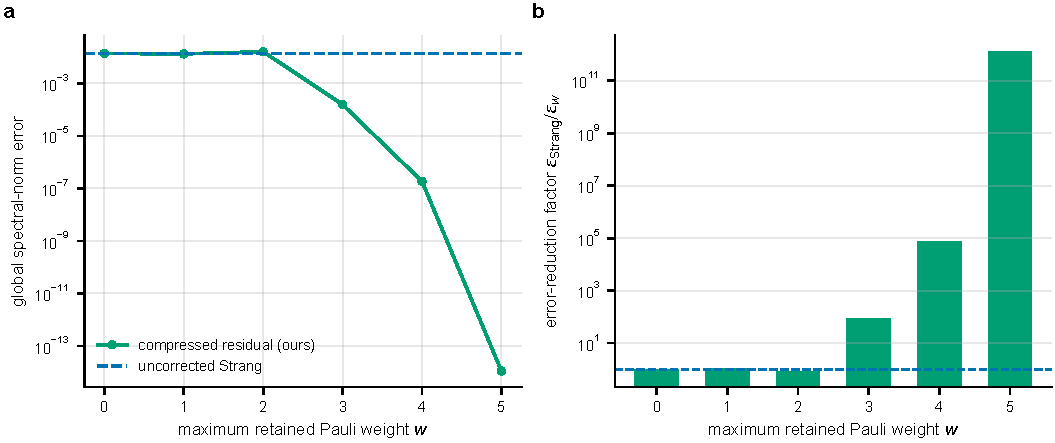
\includegraphics[width=\linewidth]{fig2_compressed_residual.pdf}
\edcaption{Compressed-residual compilation for $n=5$, $q=2$ ($J=h=1$, $t=1$, $r=10$). \textbf{a}, Spectral-norm error versus maximum retained Pauli weight $w$, against the uncorrected baseline. \textbf{b}, Improvement factor over the baseline by weight. The sharp improvement at $w=3$ is predicted by the leading-support theorem for the Strang residual (Theorem~\ref{thm:tfim-support}). All values are exact, deterministic dense-matrix computations (no sampling, hence no error bars); the $w=5$ row sits at the double-precision floor.}
\label{edfig:projected}
\end{edfigure}

\begin{edfigure}
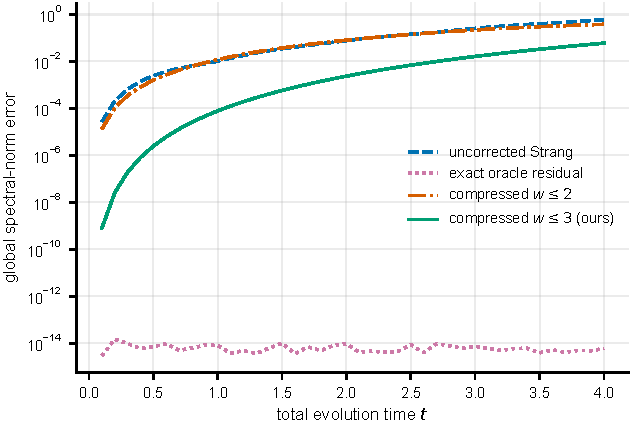
\includegraphics[width=\linewidth]{fig3_time_sweep.pdf}
\edcaption{Time-resolved correction hierarchy for $n=4$, $q=2$, $J=h=1$, and $r=10$, over $40$ total times $t\in[0.1,4.0]$. The $w\leq3$ projected residual uniformly improves the baseline in this sweep; $w\leq2$ is less reliable. Each curve is an exact, deterministic dense-matrix computation (no sampling, hence no error bars).}
\label{edfig:timesweep}
\end{edfigure}

\begin{edfigure}
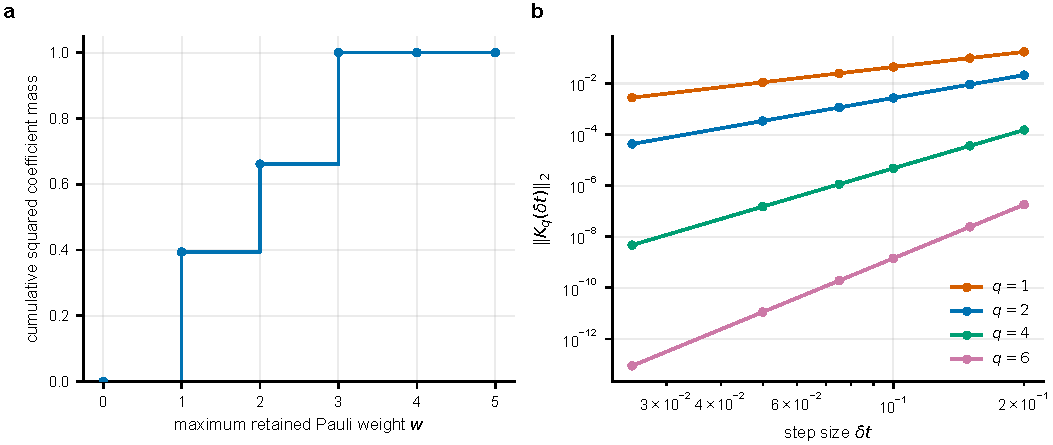
\includegraphics[width=\linewidth]{fig4_generator_structure.pdf}
\edcaption{Structure of the residual generator. \textbf{a}, Cumulative squared Pauli coefficient mass for the $n=5$, $q=2$ residual generator at $\dt=0.1$; weight three captures the dominant leading structure, while higher weights capture subleading BCH terms. \textbf{b}, Residual-generator norm $\norm{K_q(\dt)}_2$ versus step size for $n=4$ and $q=1,2,4,6$; the norm decreases rapidly with order, consistent with product-formula order conditions and Theorem~\ref{thm:small-step}. Both panels are exact, deterministic dense-matrix computations (no sampling, hence no error bars).}
\label{edfig:genstruct}
\end{edfigure}

\begin{table}[t]
\caption{\textbf{Weight-truncated residual compilation for $n=5$, $q=2$.} Parameters are $J=h=1$, $t=1$, and $r=10$. The column $w$ keeps Pauli strings of weight at most $w$ in the exact residual generator; ``projected error'' is the resulting global spectral-norm error and ``improvement'' is its ratio to the uncorrected baseline. Every entry is a single exact, deterministic dense-matrix computation (no statistical sampling, hence no uncertainty interval); the $w=5$ row is at the double-precision floor.}
\label{tab:projected-summary}
\centering
\begin{tabular}{cccc}
\toprule
$w$ & $\norm{K_q-\Pi_wK_q}_2$ & projected error & improvement\\
\midrule
0 & $3.656\times10^{-3}$ & $1.384\times10^{-2}$ & $1.00\times$\\
1 & $2.859\times10^{-3}$ & $1.330\times10^{-2}$ & $1.04\times$\\
2 & $1.949\times10^{-3}$ & $1.607\times10^{-2}$ & $0.86\times$\\
3 & $1.573\times10^{-5}$ & $1.545\times10^{-4}$ & $89.56\times$\\
4 & $1.850\times10^{-8}$ & $1.850\times10^{-7}$ & $74829.05\times$\\
5 & $1.143\times10^{-18}$ & $1.089\times10^{-14}$ & $(1.27080550904855\times10^{12})\times$\\
\bottomrule
\end{tabular}
\end{table}

\begin{table}[t]
\caption{\textbf{Per-step resource proxy.} The baseline factor count is the number of elementary $e^{-iA\tau}$ or $e^{-iB\tau}$ exponentials in the product-formula step $S_q$ of order $q$. The oracle residual construction uses one additional dense exponential for $U(\dt)$ and one dense multiplication by $S_q^\dagger$; it is not a scalable gate-level implementation. All entries are exact integer counts, not measured quantities.}
\label{tab:resources}
\centering
\begin{tabular}{cccc}
\toprule
$q$ & Suzuki factors & dense $U(\dt)$ expm & dense residual multiply\\
\midrule
1 & 2 & 1 & 1\\
2 & 3 & 1 & 1\\
4 & 15 & 1 & 1\\
6 & 75 & 1 & 1\\
8 & 375 & 1 & 1\\
\bottomrule
\end{tabular}
\end{table}

\begin{table}[t]
\caption{\textbf{Residual-generator spectral norm versus step size and product-formula order.} $\norm{K_q(\dt)}_2$ for the open-boundary \tfim{} at $n=4$, $J=h=1$, computed by dense matrix logarithm of the exact residual factor. The norm falls steeply with order $q$ and scales as $\dt^{q+1}$ at small $\dt$, the quantitative content of Theorem~\ref{thm:small-step} and Extended Data Fig.~\ref{edfig:genstruct}b. Each entry is a single exact, deterministic dense-matrix computation (no sampling, hence no uncertainty interval).}
\label{tab:generator-scaling}
\centering
\begin{tabular}{ccccc}
\toprule
$\dt$ & $\norm{K_1}_2$ & $\norm{K_2}_2$ & $\norm{K_4}_2$ & $\norm{K_6}_2$\\
\midrule
$0.025$ & $2.794\times10^{-3}$ & $4.280\times10^{-5}$ & $4.714\times10^{-9}$  & $8.777\times10^{-14}$\\
$0.050$ & $1.116\times10^{-2}$ & $3.420\times10^{-4}$ & $1.507\times10^{-7}$  & $1.122\times10^{-11}$\\
$0.075$ & $2.505\times10^{-2}$ & $1.152\times10^{-3}$ & $1.142\times10^{-6}$  & $1.915\times10^{-10}$\\
$0.100$ & $4.439\times10^{-2}$ & $2.724\times10^{-3}$ & $4.802\times10^{-6}$  & $1.432\times10^{-9}$\\
$0.150$ & $9.894\times10^{-2}$ & $9.120\times10^{-3}$ & $3.622\times10^{-5}$  & $2.433\times10^{-8}$\\
$0.200$ & $1.736\times10^{-1}$ & $2.138\times10^{-2}$ & $1.512\times10^{-4}$  & $1.809\times10^{-7}$\\
\bottomrule
\end{tabular}
\end{table}

\begin{table}[t]
\caption{\textbf{Per-size error breakdown of every correction on the disordered \tfim{}.} Global spectral-norm error at $t=1$, $\dt=0.1$ ($J_i,h_i\sim\mathcal{U}[0.5,1.5]$), reported as mean $\pm$ one standard deviation over $n_{\mathrm c}$ disordered chains (sizes and $n_{\mathrm c}$ as in Table~\ref{tab:learned-summary}). $\epsilon_{w\leq3}$ is the exact weight-$\leq3$ oracle; $\epsilon_{\mathrm{learned}}^{\,\mathrm{oracle}}$ and $\epsilon_{\mathrm{learned}}^{\,\mathrm{free}}$ are the learned corrections trained on global-oracle and on oracle-free patch labels, respectively; $\epsilon_{\mathrm{BCH}}$ is the analytic leading-order correction. The oracle-free network matches or slightly beats the oracle-trained one at every size, and both beat $\epsilon_{\mathrm{BCH}}$ by roughly $5\times$; sizes $n\geq6$ are absent from training. Best learned column in each row is bold. All values recomputed from dense matrices.}
\label{tab:learned-breakdown}
\centering
\resizebox{\textwidth}{!}{%
\begin{tabular}{cccccc}
\toprule
$n$ & regime & $\epsilon_{w\leq3}$ (oracle) & $\epsilon_{\mathrm{learned}}^{\,\mathrm{oracle}}$ & $\epsilon_{\mathrm{learned}}^{\,\mathrm{free}}$ & $\epsilon_{\mathrm{BCH}}$\\
\midrule
4  & train    & $9.43\times10^{-5} \pm 7.05\times10^{-5}$ & $3.29\times10^{-4} \pm 1.73\times10^{-4}$ & $\mathbf{2.71\times10^{-4}} \pm 2.01\times10^{-4}$ & $1.44\times10^{-3} \pm 8.00\times10^{-4}$\\
5  & train    & $1.31\times10^{-4} \pm 8.75\times10^{-5}$ & $3.79\times10^{-4} \pm 1.22\times10^{-4}$ & $\mathbf{3.63\times10^{-4}} \pm 1.42\times10^{-4}$ & $1.65\times10^{-3} \pm 7.76\times10^{-4}$\\
6  & transfer & $2.27\times10^{-4} \pm 1.16\times10^{-4}$ & $4.73\times10^{-4} \pm 1.41\times10^{-4}$ & $\mathbf{4.43\times10^{-4}} \pm 1.21\times10^{-4}$ & $2.23\times10^{-3} \pm 7.81\times10^{-4}$\\
7  & transfer & $2.75\times10^{-4} \pm 1.45\times10^{-4}$ & $6.37\times10^{-4} \pm 2.21\times10^{-4}$ & $\mathbf{5.82\times10^{-4}} \pm 2.23\times10^{-4}$ & $2.75\times10^{-3} \pm 1.03\times10^{-3}$\\
8  & transfer & $3.31\times10^{-4} \pm 1.37\times10^{-4}$ & $6.95\times10^{-4} \pm 1.69\times10^{-4}$ & $\mathbf{6.93\times10^{-4}} \pm 1.73\times10^{-4}$ & $3.29\times10^{-3} \pm 9.76\times10^{-4}$\\
9  & transfer & $3.51\times10^{-4} \pm 1.66\times10^{-4}$ & $8.10\times10^{-4} \pm 1.82\times10^{-4}$ & $\mathbf{7.40\times10^{-4}} \pm 1.59\times10^{-4}$ & $3.56\times10^{-3} \pm 1.23\times10^{-3}$\\
10 & transfer & $4.55\times10^{-4} \pm 2.07\times10^{-4}$ & $9.29\times10^{-4} \pm 1.78\times10^{-4}$ & $\mathbf{8.74\times10^{-4}} \pm 2.29\times10^{-4}$ & $4.35\times10^{-3} \pm 1.54\times10^{-3}$\\
\bottomrule
\end{tabular}%
}
\end{table}

\begin{table}[t]
\caption{\textbf{Single-step error versus step size for the learned residual at $n=6$.} Disordered open-boundary \tfim{} with $J_i,h_i\sim\mathcal{U}[0.5,1.5]$; each row is a mean $\pm$ one standard deviation over $n_{\mathrm c}=24$ disordered chains. $\epsilon_{\mathrm{Strang}}$ is the uncorrected Strang per-step spectral-norm error; $\epsilon_{w\leq3}$ is the exact weight-$\leq3$ oracle; $\epsilon_{\mathrm{learned}}$ is the oracle-free learned correction; $\epsilon_{\mathrm{BCH}}$ is the analytic leading-order ($\dt^3$) correction. As $\dt$ grows the analytic baseline degrades toward the uncorrected step while the $\dt$-conditioned learned correction tracks the oracle, quantifying Fig.~\ref{fig:learned}b. Best (smallest) correction in each row is bold; values are recomputed from dense matrices.}
\label{tab:learned-dtsweep}
\centering
\resizebox{\textwidth}{!}{%
\begin{tabular}{ccccc}
\toprule
$\dt$ & $\epsilon_{\mathrm{Strang}}$ & $\epsilon_{w\leq3}$ (oracle) & $\epsilon_{\mathrm{learned}}$ & $\epsilon_{\mathrm{BCH}}$\\
\midrule
$0.05$ & $6.71\times10^{-4} \pm 1.83\times10^{-4}$ & $\mathbf{8.88\times10^{-7}} \pm 4.72\times10^{-7}$ & $1.23\times10^{-5} \pm 6.42\times10^{-6}$ & $5.91\times10^{-5} \pm 2.08\times10^{-5}$\\
$0.10$ & $4.78\times10^{-3} \pm 1.07\times10^{-3}$ & $\mathbf{2.01\times10^{-5}} \pm 9.59\times10^{-6}$ & $6.12\times10^{-5} \pm 1.42\times10^{-5}$ & $1.08\times10^{-3} \pm 3.06\times10^{-4}$\\
$0.15$ & $1.76\times10^{-2} \pm 5.19\times10^{-3}$ & $\mathbf{1.95\times10^{-4}} \pm 1.15\times10^{-4}$ & $3.07\times10^{-4} \pm 1.53\times10^{-4}$ & $6.74\times10^{-3} \pm 2.68\times10^{-3}$\\
$0.20$ & $3.75\times10^{-2} \pm 1.12\times10^{-2}$ & $\mathbf{6.85\times10^{-4}} \pm 3.90\times10^{-4}$ & $8.99\times10^{-4} \pm 4.01\times10^{-4}$ & $1.95\times10^{-2} \pm 7.65\times10^{-3}$\\
$0.25$ & $7.10\times10^{-2} \pm 2.03\times10^{-2}$ & $\mathbf{1.87\times10^{-3}} \pm 9.01\times10^{-4}$ & $2.33\times10^{-3} \pm 9.31\times10^{-4}$ & $4.65\times10^{-2} \pm 1.68\times10^{-2}$\\
$0.30$ & $1.33\times10^{-1} \pm 3.60\times10^{-2}$ & $\mathbf{5.23\times10^{-3}} \pm 3.11\times10^{-3}$ & $6.24\times10^{-3} \pm 3.31\times10^{-3}$ & $1.07\times10^{-1} \pm 4.00\times10^{-2}$\\
\bottomrule
\end{tabular}%
}
\end{table}

The per-size breakdown of every correction (Extended Data Table~\ref{tab:learned-breakdown}) makes the overlap of the oracle-trained and oracle-free learned curves in Fig.~\ref{fig:learned}a quantitative: at every size the oracle-free network matches or slightly improves on the oracle-trained one and both sit about a factor of five below the analytic leading-order correction, while staying within a small constant factor of the exact weight-$\leq3$ oracle. The single-step step-size sweep at $n=6$ (Extended Data Table~\ref{tab:learned-dtsweep}) tabulates the numbers behind Fig.~\ref{fig:learned}b: the analytic $\dt^3$ correction degrades from an $11\times$ improvement over the uncorrected step at $\dt=0.05$ to only $1.24\times$ at $\dt=0.30$, whereas the $\dt$-conditioned learned correction stays close to the exact oracle, closing from about a factor of fourteen at $\dt=0.05$ to within roughly $20\%$ at $\dt=0.30$ and remaining far below the analytic baseline throughout. The residual-generator norms in Extended Data Table~\ref{tab:generator-scaling} confirm the order scaling underlying Theorem~\ref{thm:small-step}: increasing the order from $q=1$ to $q=6$ shrinks $\norm{K_q(0.1)}_2$ from $4.44\times10^{-2}$ to $1.43\times10^{-9}$.

\subsection*{Supplementary theory: detailed BCH support analysis for the TFIM}
\label{app:bch}

The support theorem in the main text is intentionally stated without relying on exact BCH coefficients. This appendix gives the more explicit structure. For Strang splitting, $S_2(\dt)=e^{-iB\dt/2}e^{-iA\dt}e^{-iB\dt/2}$, the logarithm has the form $\log S_2(\dt)=-i(A+B)\dt+\dt^3\Gamma_3+O(\dt^5)$, where $\Gamma_3$ is a linear combination of $[A,[A,B]]$ and $[B,[A,B]]$. The absence of an even power follows from time-reversal symmetry of the Strang formula. The residual is $R_2(\dt)=e^{-i(A+B)\dt}S_2(\dt)^\dagger$, and the leading residual generator cancels the leading logarithmic defect, so $K_2(\dt)=\dt^3K_2^{(3)}+O(\dt^5)$, where $K_2^{(3)}$ is a real linear combination of $i[A,[A,B]]$ and $i[B,[A,B]]$ after accounting for the anti-Hermitian nature of commutators of Hermitian matrices.

For the \tfim{}, write $A_e=JZ_jZ_{j+1}$ and $B_v=hX_v$. The elementary commutator is $[A_e,B_v]=0$ if $v\notin e$. If $v=j$, then $[Z_jZ_{j+1},X_j]=2iY_jZ_{j+1}$, and if $v=j+1$, then $[Z_jZ_{j+1},X_{j+1}]=2iZ_jY_{j+1}$. Thus $[A,B]$ is a sum of weight-two Pauli strings on nearest-neighbor edges. Next consider $[B,[A,B]]$: a term $[B_{v'},[A_e,B_v]]$ is nonzero only if $v'$ lies in the support of $[A_e,B_v]$, which is the same edge $e$; the resulting Pauli string remains supported on that edge and has weight at most two, for example $[X_j,Y_jZ_{j+1}]=2iZ_jZ_{j+1}$ and $[X_{j+1},Y_jZ_{j+1}]=-2iY_jY_{j+1}$. Now consider $[A,[A,B]]$: a term $[A_{e'},[A_e,B_v]]$ is nonzero only if $e'$ overlaps the support of $[A_e,B_v]$. In a one-dimensional nearest-neighbor chain, the union of two overlapping edges contains at most three sites, $(j-1,j,j+1)$ or $(j,j+1,j+2)$. Therefore every nonzero Pauli string in $[A,[A,B]]$ has weight at most three, proving that the leading Strang residual generator is contained in $\cB_3$. The same proof strategy extends to other local Hamiltonians: if the interaction hypergraph has local terms of diameter at most $r_0$, then an $m$-fold nested commutator can only grow along overlapping local supports, connecting residual-generator compression to locality bounds and Lieb--Robinson ideas~\cite{lieb1972,tran2020}.

\subsection*{Supplementary theory: projection formulas and diagnostic quantities}
\label{app:projection}

For $n$ qubits, the Pauli group modulo phases gives $4^n$ Hermitian strings satisfying $\Tr(PQ)=2^n\delta_{P,Q}$. Every Hermitian matrix $K$ has an expansion $K=\sum_{P\in\cP_n} c_P P$ with $c_P=\Tr(PK)/2^n$, squared Frobenius norm $\norm{K}_F^2=2^n\sum_{P\in\cP_n}\abs{c_P}^2$, and cumulative coefficient mass (plotted in Extended Data Fig.~\ref{edfig:genstruct}a) $M(w)=\sum_{\operatorname{wt}(P)\leq w}\abs{c_P}^2/\sum_{P\in\cP_n}\abs{c_P}^2$. For the $n=5$, $q=2$, $\dt=0.1$ run, the generated squared coefficient masses by weight are $M_0'=3.598\times10^{-33}$, $M_1'=1.466\times10^{-6}$, $M_2'=9.973\times10^{-7}$, $M_3'=1.262\times10^{-6}$, $M_4'=1.235\times10^{-10}$, and $M_5'=3.413\times10^{-16}$. Although the weight-four mass is small in Frobenius terms, it can still matter for spectral-norm accuracy after repeated steps, which is why Extended Data Table~\ref{tab:projected-summary} shows a large improvement from $w=3$ to $w=4$.

\subsection*{Supplementary theory: finite-precision interpretation}
\label{app:finite-precision}

The exact residual theorem is an algebraic identity. In floating-point arithmetic, the computed residual is $\widetilde R_q=\operatorname{fl}\{\widetilde U(\dt)\widetilde S_q(\dt)^\dagger\}$ and the computed corrected step is $\widetilde G_q=\operatorname{fl}\{\widetilde R_q\widetilde S_q\}$. Round-off enters through every matrix exponential and multiplication. This explains why the $q=8$ baseline, already extremely accurate at $\dt=0.1$, can appear slightly more accurate than the oracle residual in Table~\ref{tab:error-summary}: the theorem says the exact-arithmetic error is zero, while the table reports floating-point evaluations of different arithmetic circuits. For low and moderate order, the product-formula error dominates round-off and oracle \rgtc{} gives many orders of magnitude improvement; for very high order at small step size, product-formula error can be below or comparable to double-precision round-off, so differences at $10^{-13}$ are not physically meaningful; projected residual experiments should be judged at error levels well above round-off, such as the $w=3$ and $w=4$ results in Extended Data Table~\ref{tab:projected-summary}.

\subsection*{Supplementary: reproducibility checklist}
\label{app:repro}

A reproducible implementation should verify $\norm{S_q^\dagger S_q-\id}_2<10^{-12}$ for every tested $q$, $n$, and $\dt$; verify $\norm{R_q^\dagger R_q-\id}_2<10^{-12}$ for every oracle residual; verify $\norm{R_qS_q-U(\dt)}_2<10^{-12}$ for small and moderate orders; save raw CSV or JSON data before plotting; make plots only from saved raw data, not from hard-coded arrays; record package versions and BLAS backend information; use deterministic parameter grids or fixed random seeds; and include tests that fail if a citation key in \texttt{main.tex} is missing from \texttt{refs.bib}. These checks are especially important if the code is ported to GPU backends, where matrix-exponential implementations and floating-point accumulation order may differ from CPU reference values.

\subsection*{Supplementary: possible extensions}
\label{app:extensions}

The residual-generator framework suggests several concrete research extensions. A \emph{BCH residual compiler} derives explicit nested-commutator formulas for $K_q$ through a target order and implements $e^{-iK_q^{\mathrm{BCH}}}$ as a short product formula; Theorems~\ref{thm:residual-stability} and~\ref{thm:duhamel} convert truncation error into global simulation error. A \emph{variational residual compiler} uses the oracle residual on small systems as a target for a parameterized local circuit $V(\theta)$, with loss $\norm{V(\theta)-R_q}_F^2$, local Pauli-shadow loss, or state-averaged infidelity, and the stability theorem provides the operator-norm target. An \emph{operator-learning residual compiler} is realized in Sec.~\ref{sec:learned} for the Strang \tfim{}, learning the step-size-conditioned local weight-$\leq3$ coefficients of $K_2$ with a single size-transferable network trained from oracle-free local patches; natural continuations extend the local templates to other lattices and higher orders, replace patch labels with classical-shadow or commutator estimates on hardware, and compile the learned generator $e^{-i\widehat K_q}$ into native gates using Theorems~\ref{thm:residual-stability} and~\ref{thm:duhamel} as the operator-norm target. A \emph{GPU-accelerated benchmark generator} uses CPU dense simulation as a correctness reference, then ports parameter sweeps and Pauli projections to batched GPU kernels, keeping output tolerance-comparable to the CPU reference and always regenerating raw data before producing figures.

\end{document}
